\section{Complete Primary and Supporting Results}
\subsection{Complete final primary results}
Tables below retain every ordered pair and every registered endpoint. Shared/disjoint ranking points use examination means and fixed A-error or condition-specific paired error as explicitly labeled. No null or negative pair is dropped. The acquired-only tables retain all four strata, and the fixed-context table retains every amplitude. Case/context-level values, including all individual approximation failures, are in the corresponding CSVs.
\begin{table*}[t]\centering\small
\caption{fastMRI: observable fraction. All ordered pairs; simultaneous family size 20.}
\begin{tabular}{llrrr}\toprule Reference A & Companion B & Shared & Disjoint & Disjoint minus shared [simultaneous 95\% CI]\\\midrule
HAT & SWINIR & 0.048 & 0.208 & 0.160 [0.146,0.174] \\
HAT & I3NET & 0.131 & 0.229 & 0.098 [0.088,0.108] \\
HAT & SAINT & 0.079 & 0.209 & 0.130 [0.116,0.143] \\
HAT & CYCLEINR & 0.165 & 0.281 & 0.116 [0.103,0.128] \\
SWINIR & HAT & 0.048 & 0.205 & 0.157 [0.143,0.170] \\
SWINIR & I3NET & 0.148 & 0.234 & 0.086 [0.075,0.098] \\
SWINIR & SAINT & 0.100 & 0.209 & 0.109 [0.093,0.125] \\
SWINIR & CYCLEINR & 0.139 & 0.250 & 0.111 [0.094,0.127] \\
I3NET & HAT & 0.131 & 0.220 & 0.089 [0.076,0.101] \\
I3NET & SWINIR & 0.148 & 0.225 & 0.077 [0.064,0.091] \\
I3NET & SAINT & 0.101 & 0.208 & 0.107 [0.097,0.117] \\
I3NET & CYCLEINR & 0.238 & 0.301 & 0.062 [0.052,0.072] \\
SAINT & HAT & 0.079 & 0.206 & 0.127 [0.112,0.141] \\
SAINT & SWINIR & 0.100 & 0.209 & 0.108 [0.092,0.125] \\
SAINT & I3NET & 0.101 & 0.212 & 0.111 [0.101,0.122] \\
SAINT & CYCLEINR & 0.208 & 0.285 & 0.078 [0.065,0.090] \\
CYCLEINR & HAT & 0.165 & 0.277 & 0.112 [0.095,0.129] \\
CYCLEINR & SWINIR & 0.139 & 0.254 & 0.115 [0.094,0.135] \\
CYCLEINR & I3NET & 0.238 & 0.306 & 0.068 [0.054,0.082] \\
CYCLEINR & SAINT & 0.208 & 0.283 & 0.076 [0.057,0.094] \\
\bottomrule\end{tabular}\end{table*}
\begin{table*}[t]\centering\small
\caption{fastMRI: error alignment. All ordered pairs; simultaneous family size 20.}
\begin{tabular}{llrrr}\toprule Reference A & Companion B & Shared & Disjoint & Disjoint minus shared [simultaneous 95\% CI]\\\midrule
HAT & SWINIR & 0.906 & 0.586 & -0.320 [-0.348,-0.292] \\
HAT & I3NET & 0.746 & 0.552 & -0.195 [-0.216,-0.174] \\
HAT & SAINT & 0.845 & 0.587 & -0.258 [-0.286,-0.231] \\
HAT & CYCLEINR & 0.702 & 0.462 & -0.240 [-0.265,-0.216] \\
SWINIR & HAT & 0.906 & 0.594 & -0.312 [-0.339,-0.285] \\
SWINIR & I3NET & 0.720 & 0.547 & -0.174 [-0.198,-0.149] \\
SWINIR & SAINT & 0.808 & 0.591 & -0.217 [-0.249,-0.185] \\
SWINIR & CYCLEINR & 0.746 & 0.520 & -0.226 [-0.258,-0.193] \\
I3NET & HAT & 0.746 & 0.567 & -0.180 [-0.205,-0.154] \\
I3NET & SWINIR & 0.720 & 0.561 & -0.159 [-0.186,-0.132] \\
I3NET & SAINT & 0.802 & 0.588 & -0.214 [-0.233,-0.194] \\
I3NET & CYCLEINR & 0.575 & 0.439 & -0.136 [-0.156,-0.115] \\
SAINT & HAT & 0.845 & 0.591 & -0.254 [-0.282,-0.226] \\
SAINT & SWINIR & 0.808 & 0.588 & -0.220 [-0.252,-0.188] \\
SAINT & I3NET & 0.802 & 0.580 & -0.222 [-0.243,-0.201] \\
SAINT & CYCLEINR & 0.628 & 0.463 & -0.165 [-0.191,-0.139] \\
CYCLEINR & HAT & 0.702 & 0.471 & -0.231 [-0.267,-0.195] \\
CYCLEINR & SWINIR & 0.746 & 0.514 & -0.232 [-0.273,-0.190] \\
CYCLEINR & I3NET & 0.575 & 0.431 & -0.144 [-0.172,-0.116] \\
CYCLEINR & SAINT & 0.628 & 0.469 & -0.159 [-0.197,-0.122] \\
\bottomrule\end{tabular}\end{table*}
\begin{table*}[t]\centering\small
\caption{fastMRI: disagreement MAE. All ordered pairs; simultaneous family size 20.}
\begin{tabular}{llrrr}\toprule Reference A & Companion B & Shared & Disjoint & Disjoint minus shared [simultaneous 95\% CI]\\\midrule
HAT & SWINIR & 32.561 & 68.966 & 36.405 [30.512,42.297] \\
HAT & I3NET & 49.666 & 64.623 & 14.957 [12.590,17.323] \\
HAT & SAINT & 39.651 & 63.827 & 24.176 [19.954,28.398] \\
HAT & CYCLEINR & 69.079 & 97.251 & 28.172 [24.182,32.162] \\
SWINIR & HAT & 32.561 & 68.394 & 35.833 [30.035,41.630] \\
SWINIR & I3NET & 54.252 & 67.907 & 13.655 [11.270,16.040] \\
SWINIR & SAINT & 45.376 & 66.128 & 20.751 [16.576,24.926] \\
SWINIR & CYCLEINR & 62.572 & 93.295 & 30.723 [25.738,35.707] \\
I3NET & HAT & 49.666 & 64.061 & 14.394 [11.762,17.027] \\
I3NET & SWINIR & 54.252 & 67.148 & 12.896 [10.376,15.416] \\
I3NET & SAINT & 41.630 & 58.546 & 16.915 [14.279,19.552] \\
I3NET & CYCLEINR & 82.091 & 94.770 & 12.678 [10.256,15.101] \\
SAINT & HAT & 39.651 & 63.958 & 24.306 [20.003,28.610] \\
SAINT & SWINIR & 45.376 & 66.666 & 21.290 [17.164,25.415] \\
SAINT & I3NET & 41.630 & 58.688 & 17.057 [14.337,19.778] \\
SAINT & CYCLEINR & 77.427 & 94.594 & 17.167 [14.113,20.221] \\
CYCLEINR & HAT & 69.079 & 95.043 & 25.964 [21.814,30.114] \\
CYCLEINR & SWINIR & 62.572 & 92.557 & 29.984 [24.559,35.409] \\
CYCLEINR & I3NET & 82.091 & 93.957 & 11.866 [9.357,14.375] \\
CYCLEINR & SAINT & 77.427 & 92.818 & 15.391 [12.023,18.758] \\
\bottomrule\end{tabular}\end{table*}
\begin{table*}[t]\centering\small
\caption{fastMRI: fixed-reference examination ranking. All ordered pairs; simultaneous family size 20.}
\begin{tabular}{llrrr}\toprule Reference A & Companion B & Shared & Disjoint & Disjoint minus shared [simultaneous 95\% CI]\\\midrule
HAT & SWINIR & 0.930 & 0.963 & 0.033 [-0.157,0.223] \\
HAT & I3NET & 0.954 & 0.968 & 0.014 [-0.100,0.128] \\
HAT & SAINT & 0.963 & 0.965 & 0.002 [-0.131,0.134] \\
HAT & CYCLEINR & 0.810 & 0.881 & 0.070 [-0.118,0.259] \\
SWINIR & HAT & 0.957 & 0.974 & 0.017 [-0.135,0.168] \\
SWINIR & I3NET & 0.971 & 0.980 & 0.009 [-0.090,0.108] \\
SWINIR & SAINT & 0.962 & 0.964 & 0.003 [-0.163,0.168] \\
SWINIR & CYCLEINR & 0.770 & 0.908 & 0.137 [-0.149,0.424] \\
I3NET & HAT & 0.919 & 0.953 & 0.034 [-0.110,0.178] \\
I3NET & SWINIR & 0.911 & 0.945 & 0.034 [-0.139,0.207] \\
I3NET & SAINT & 0.957 & 0.974 & 0.017 [-0.090,0.125] \\
I3NET & CYCLEINR & 0.710 & 0.821 & 0.111 [-0.117,0.340] \\
SAINT & HAT & 0.955 & 0.968 & 0.013 [-0.101,0.127] \\
SAINT & SWINIR & 0.931 & 0.968 & 0.037 [-0.136,0.209] \\
SAINT & I3NET & 0.968 & 0.965 & -0.003 [-0.116,0.111] \\
SAINT & CYCLEINR & 0.830 & 0.858 & 0.028 [-0.156,0.211] \\
CYCLEINR & HAT & 0.965 & 0.983 & 0.018 [-0.110,0.146] \\
CYCLEINR & SWINIR & 0.938 & 0.976 & 0.037 [-0.139,0.214] \\
CYCLEINR & I3NET & 0.965 & 0.990 & 0.025 [-0.073,0.123] \\
CYCLEINR & SAINT & 0.980 & 0.984 & 0.004 [-0.097,0.105] \\
\bottomrule\end{tabular}\end{table*}
\begin{table*}[t]\centering\small
\caption{fastMRI: condition-specific paired-error examination ranking. All ordered pairs; simultaneous family size 20.}
\begin{tabular}{llrrr}\toprule Reference A & Companion B & Shared & Disjoint & Disjoint minus shared [simultaneous 95\% CI]\\\midrule
HAT & SWINIR & 0.943 & 0.964 & 0.021 [-0.160,0.201] \\
HAT & I3NET & 0.931 & 0.972 & 0.041 [-0.094,0.175] \\
HAT & SAINT & 0.957 & 0.965 & 0.008 [-0.100,0.115] \\
HAT & CYCLEINR & 0.934 & 0.973 & 0.039 [-0.081,0.159] \\
SWINIR & HAT & 0.943 & 0.972 & 0.029 [-0.140,0.197] \\
SWINIR & I3NET & 0.932 & 0.961 & 0.029 [-0.120,0.178] \\
SWINIR & SAINT & 0.947 & 0.968 & 0.021 [-0.147,0.189] \\
SWINIR & CYCLEINR & 0.886 & 0.977 & 0.090 [-0.126,0.307] \\
I3NET & HAT & 0.931 & 0.974 & 0.043 [-0.098,0.183] \\
I3NET & SWINIR & 0.932 & 0.973 & 0.041 [-0.130,0.212] \\
I3NET & SAINT & 0.964 & 0.982 & 0.017 [-0.104,0.139] \\
I3NET & CYCLEINR & 0.910 & 0.957 & 0.047 [-0.099,0.193] \\
SAINT & HAT & 0.957 & 0.966 & 0.009 [-0.111,0.128] \\
SAINT & SWINIR & 0.947 & 0.971 & 0.024 [-0.130,0.178] \\
SAINT & I3NET & 0.964 & 0.984 & 0.020 [-0.093,0.133] \\
SAINT & CYCLEINR & 0.948 & 0.972 & 0.024 [-0.099,0.147] \\
CYCLEINR & HAT & 0.934 & 0.983 & 0.050 [-0.076,0.175] \\
CYCLEINR & SWINIR & 0.886 & 0.988 & 0.102 [-0.089,0.293] \\
CYCLEINR & I3NET & 0.910 & 0.986 & 0.076 [-0.082,0.233] \\
CYCLEINR & SAINT & 0.948 & 0.982 & 0.034 [-0.102,0.170] \\
\bottomrule\end{tabular}\end{table*}
\begin{table*}[t]\centering\small
\caption{IXI: observable fraction. All ordered pairs; simultaneous family size 20.}
\begin{tabular}{llrrr}\toprule Reference A & Companion B & Shared & Disjoint & Disjoint minus shared [simultaneous 95\% CI]\\\midrule
HAT & SWINIR & 0.023 & 0.309 & 0.285 [0.278,0.292] \\
HAT & I3NET & 0.144 & 0.328 & 0.183 [0.173,0.193] \\
HAT & SAINT & 0.036 & 0.312 & 0.275 [0.268,0.283] \\
HAT & CYCLEINR & 0.125 & 0.337 & 0.212 [0.206,0.218] \\
SWINIR & HAT & 0.023 & 0.308 & 0.285 [0.278,0.292] \\
SWINIR & I3NET & 0.149 & 0.331 & 0.183 [0.173,0.193] \\
SWINIR & SAINT & 0.035 & 0.316 & 0.281 [0.274,0.289] \\
SWINIR & CYCLEINR & 0.113 & 0.337 & 0.224 [0.218,0.230] \\
I3NET & HAT & 0.144 & 0.324 & 0.180 [0.169,0.191] \\
I3NET & SWINIR & 0.149 & 0.328 & 0.180 [0.169,0.191] \\
I3NET & SAINT & 0.149 & 0.329 & 0.180 [0.168,0.191] \\
I3NET & CYCLEINR & 0.237 & 0.368 & 0.131 [0.121,0.141] \\
SAINT & HAT & 0.036 & 0.311 & 0.275 [0.268,0.282] \\
SAINT & SWINIR & 0.035 & 0.316 & 0.281 [0.274,0.288] \\
SAINT & I3NET & 0.149 & 0.332 & 0.182 [0.172,0.193] \\
SAINT & CYCLEINR & 0.107 & 0.333 & 0.226 [0.220,0.232] \\
CYCLEINR & HAT & 0.125 & 0.336 & 0.211 [0.206,0.217] \\
CYCLEINR & SWINIR & 0.113 & 0.336 & 0.223 [0.218,0.229] \\
CYCLEINR & I3NET & 0.237 & 0.368 & 0.132 [0.122,0.141] \\
CYCLEINR & SAINT & 0.107 & 0.332 & 0.226 [0.220,0.231] \\
\bottomrule\end{tabular}\end{table*}
\begin{table*}[t]\centering\small
\caption{IXI: error alignment. All ordered pairs; simultaneous family size 20.}
\begin{tabular}{llrrr}\toprule Reference A & Companion B & Shared & Disjoint & Disjoint minus shared [simultaneous 95\% CI]\\\midrule
HAT & SWINIR & 0.953 & 0.392 & -0.562 [-0.577,-0.547] \\
HAT & I3NET & 0.751 & 0.376 & -0.375 [-0.394,-0.356] \\
HAT & SAINT & 0.928 & 0.385 & -0.543 [-0.558,-0.528] \\
HAT & CYCLEINR & 0.772 & 0.340 & -0.432 [-0.445,-0.419] \\
SWINIR & HAT & 0.953 & 0.393 & -0.561 [-0.576,-0.545] \\
SWINIR & I3NET & 0.744 & 0.369 & -0.375 [-0.393,-0.356] \\
SWINIR & SAINT & 0.931 & 0.377 & -0.554 [-0.569,-0.539] \\
SWINIR & CYCLEINR & 0.795 & 0.339 & -0.456 [-0.470,-0.443] \\
I3NET & HAT & 0.751 & 0.374 & -0.377 [-0.398,-0.356] \\
I3NET & SWINIR & 0.744 & 0.367 & -0.377 [-0.398,-0.356] \\
I3NET & SAINT & 0.744 & 0.366 & -0.377 [-0.399,-0.356] \\
I3NET & CYCLEINR & 0.598 & 0.302 & -0.296 [-0.317,-0.276] \\
SAINT & HAT & 0.928 & 0.387 & -0.541 [-0.556,-0.526] \\
SAINT & SWINIR & 0.931 & 0.378 & -0.553 [-0.568,-0.538] \\
SAINT & I3NET & 0.744 & 0.369 & -0.375 [-0.394,-0.356] \\
SAINT & CYCLEINR & 0.807 & 0.348 & -0.459 [-0.473,-0.446] \\
CYCLEINR & HAT & 0.772 & 0.348 & -0.424 [-0.436,-0.412] \\
CYCLEINR & SWINIR & 0.795 & 0.347 & -0.448 [-0.460,-0.437] \\
CYCLEINR & I3NET & 0.598 & 0.310 & -0.288 [-0.305,-0.271] \\
CYCLEINR & SAINT & 0.807 & 0.355 & -0.452 [-0.464,-0.440] \\
\bottomrule\end{tabular}\end{table*}
\begin{table*}[t]\centering\small
\caption{IXI: disagreement MAE. All ordered pairs; simultaneous family size 20.}
\begin{tabular}{llrrr}\toprule Reference A & Companion B & Shared & Disjoint & Disjoint minus shared [simultaneous 95\% CI]\\\midrule
HAT & SWINIR & 12.802 & 47.636 & 34.834 [29.981,39.688] \\
HAT & I3NET & 25.363 & 42.163 & 16.799 [14.023,19.575] \\
HAT & SAINT & 16.663 & 48.019 & 31.356 [26.933,35.778] \\
HAT & CYCLEINR & 32.883 & 58.337 & 25.454 [21.767,29.141] \\
SWINIR & HAT & 12.802 & 47.512 & 34.710 [29.891,39.529] \\
SWINIR & I3NET & 26.156 & 42.728 & 16.572 [13.834,19.310] \\
SWINIR & SAINT & 16.435 & 48.484 & 32.049 [27.541,36.557] \\
SWINIR & CYCLEINR & 30.953 & 58.390 & 27.438 [23.541,31.335] \\
I3NET & HAT & 25.363 & 41.824 & 16.461 [13.620,19.302] \\
I3NET & SWINIR & 26.156 & 42.482 & 16.325 [13.511,19.140] \\
I3NET & SAINT & 27.134 & 42.754 & 15.621 [12.861,18.381] \\
I3NET & CYCLEINR & 42.289 & 54.835 & 12.546 [10.251,14.841] \\
SAINT & HAT & 16.663 & 47.983 & 31.320 [26.922,35.718] \\
SAINT & SWINIR & 16.435 & 48.541 & 32.106 [27.598,36.614] \\
SAINT & I3NET & 27.134 & 43.073 & 15.939 [13.263,18.616] \\
SAINT & CYCLEINR & 30.820 & 58.205 & 27.386 [23.449,31.323] \\
CYCLEINR & HAT & 32.883 & 58.318 & 25.434 [21.767,29.101] \\
CYCLEINR & SWINIR & 30.953 & 58.441 & 27.489 [23.586,31.392] \\
CYCLEINR & I3NET & 42.289 & 54.936 & 12.647 [10.444,14.851] \\
CYCLEINR & SAINT & 30.820 & 58.206 & 27.386 [23.455,31.317] \\
\bottomrule\end{tabular}\end{table*}
\begin{table*}[t]\centering\small
\caption{IXI: fixed-reference examination ranking. All ordered pairs; simultaneous family size 20.}
\begin{tabular}{llrrr}\toprule Reference A & Companion B & Shared & Disjoint & Disjoint minus shared [simultaneous 95\% CI]\\\midrule
HAT & SWINIR & 0.964 & 0.992 & 0.028 [0.001,0.056] \\
HAT & I3NET & 0.969 & 0.993 & 0.025 [-0.003,0.053] \\
HAT & SAINT & 0.958 & 0.991 & 0.033 [0.002,0.064] \\
HAT & CYCLEINR & 0.938 & 0.983 & 0.045 [0.011,0.078] \\
SWINIR & HAT & 0.965 & 0.993 & 0.028 [0.001,0.055] \\
SWINIR & I3NET & 0.970 & 0.994 & 0.024 [-0.003,0.051] \\
SWINIR & SAINT & 0.961 & 0.992 & 0.031 [0.003,0.059] \\
SWINIR & CYCLEINR & 0.939 & 0.983 & 0.044 [0.013,0.076] \\
I3NET & HAT & 0.937 & 0.987 & 0.050 [0.002,0.098] \\
I3NET & SWINIR & 0.938 & 0.986 & 0.049 [0.002,0.095] \\
I3NET & SAINT & 0.932 & 0.986 & 0.053 [0.004,0.103] \\
I3NET & CYCLEINR & 0.912 & 0.970 & 0.058 [0.008,0.108] \\
SAINT & HAT & 0.962 & 0.993 & 0.031 [0.002,0.061] \\
SAINT & SWINIR & 0.964 & 0.993 & 0.030 [0.003,0.056] \\
SAINT & I3NET & 0.967 & 0.994 & 0.027 [-0.002,0.057] \\
SAINT & CYCLEINR & 0.946 & 0.985 & 0.040 [0.010,0.069] \\
CYCLEINR & HAT & 0.964 & 0.993 & 0.029 [0.004,0.054] \\
CYCLEINR & SWINIR & 0.964 & 0.993 & 0.030 [0.005,0.054] \\
CYCLEINR & I3NET & 0.968 & 0.994 & 0.025 [-0.001,0.052] \\
CYCLEINR & SAINT & 0.967 & 0.993 & 0.026 [0.003,0.049] \\
\bottomrule\end{tabular}\end{table*}
\begin{table*}[t]\centering\small
\caption{IXI: condition-specific paired-error examination ranking. All ordered pairs; simultaneous family size 20.}
\begin{tabular}{llrrr}\toprule Reference A & Companion B & Shared & Disjoint & Disjoint minus shared [simultaneous 95\% CI]\\\midrule
HAT & SWINIR & 0.964 & 0.994 & 0.030 [0.004,0.057] \\
HAT & I3NET & 0.958 & 0.993 & 0.036 [0.002,0.069] \\
HAT & SAINT & 0.960 & 0.994 & 0.034 [0.004,0.064] \\
HAT & CYCLEINR & 0.954 & 0.993 & 0.039 [0.009,0.068] \\
SWINIR & HAT & 0.964 & 0.994 & 0.030 [0.004,0.057] \\
SWINIR & I3NET & 0.959 & 0.994 & 0.035 [0.003,0.067] \\
SWINIR & SAINT & 0.962 & 0.994 & 0.032 [0.005,0.059] \\
SWINIR & CYCLEINR & 0.953 & 0.992 & 0.039 [0.011,0.067] \\
I3NET & HAT & 0.958 & 0.995 & 0.037 [0.003,0.071] \\
I3NET & SWINIR & 0.959 & 0.995 & 0.036 [0.004,0.068] \\
I3NET & SAINT & 0.955 & 0.995 & 0.040 [0.005,0.075] \\
I3NET & CYCLEINR & 0.954 & 0.992 & 0.038 [0.005,0.071] \\
SAINT & HAT & 0.960 & 0.995 & 0.034 [0.004,0.064] \\
SAINT & SWINIR & 0.962 & 0.995 & 0.032 [0.005,0.060] \\
SAINT & I3NET & 0.955 & 0.993 & 0.038 [0.004,0.073] \\
SAINT & CYCLEINR & 0.958 & 0.993 & 0.035 [0.008,0.061] \\
CYCLEINR & HAT & 0.954 & 0.992 & 0.038 [0.010,0.066] \\
CYCLEINR & SWINIR & 0.953 & 0.992 & 0.039 [0.012,0.065] \\
CYCLEINR & I3NET & 0.954 & 0.990 & 0.036 [0.005,0.067] \\
CYCLEINR & SAINT & 0.958 & 0.992 & 0.033 [0.009,0.058] \\
\bottomrule\end{tabular}\end{table*}

\begin{table*}[t]
\centering\small
\caption{Acquired-only neural influence. Beyond-count and fixed-one-anchor estimates have simultaneous 95\% intervals across both models, separately by cohort/endpoint. Stability is the minimum of three amplitude/sign correlations; the historical per-stratum threshold is .85.}
\label{tab:neural}
\setlength{\tabcolsep}{5pt}
\begin{tabular}{llrrr}\toprule
Cohort & Model & $|\rho_I|-|\rho_{count}|$ [CI] & Fixed-count partial $\rho$ [CI] & Minimum stability / status\\\midrule
IXI & HAT & 0.098 [0.090,0.106] & 0.270 [0.194,0.345] & 0.930 / PASS \\
IXI & SwinIR & 0.093 [0.084,0.103] & 0.265 [0.195,0.334] & 0.880 / PASS \\
fastMRI & HAT & 0.103 [0.089,0.118] & 0.474 [0.321,0.627] & 0.964 / PASS \\
fastMRI & SwinIR & 0.093 [0.080,0.106] & 0.365 [0.216,0.514] & 0.942 / PASS \\
\bottomrule\end{tabular}
\end{table*}

\begin{table*}[t]\centering\small\caption{All acquired-only amplitude/sign stability checks against +.01. The per-stratum threshold is .85; the original six-stratum aggregate gate is NA.}\begin{tabular}{llrrl}\toprule Cohort & Model & Alternative amplitude & Rank stability & Status\\\midrule
fastmri & HAT & 0.005 & 0.9855 & PASS \\
fastmri & HAT & 0.02 & 0.9643 & PASS \\
fastmri & HAT & -0.01 & 0.9726 & PASS \\
fastmri & SWINIR & 0.005 & 0.9789 & PASS \\
fastmri & SWINIR & 0.02 & 0.9421 & PASS \\
fastmri & SWINIR & -0.01 & 0.9776 & PASS \\
ixi & HAT & 0.005 & 0.9298 & PASS \\
ixi & HAT & 0.02 & 0.9576 & PASS \\
ixi & HAT & -0.01 & 0.9348 & PASS \\
ixi & SWINIR & 0.005 & 0.8803 & PASS \\
ixi & SWINIR & 0.02 & 0.9505 & PASS \\
ixi & SWINIR & -0.01 & 0.9113 & PASS \\
\bottomrule\end{tabular}\end{table*}
\begin{table*}[t]\centering\small\caption{Every fixed-context neural amplitude. Effects are in native squared-intensity units; intervals are simultaneous over eight model/amplitude contrasts. Relative approximation error uses the fixed .0025 prediction as denominator.}\begin{tabular}{llrrr}\toprule Model & Amplitude & Observed mean [95\% CI] & Fixed-linear mean & Median relative error\\\midrule
HAT & 0.0025 & -1.803 [-2.835,-0.771] & -1.792 & 1.90\% \\
HAT & 0.005 & -7.350 [-11.630,-3.069] & -7.169 & 5.75\% \\
HAT & 0.01 & -28.758 [-45.345,-12.172] & -28.676 & 8.92\% \\
HAT & 0.02 & -110.005 [-173.455,-46.556] & -114.705 & 10.61\% \\
SWINIR & 0.0025 & -1.502 [-2.366,-0.639] & -1.515 & 2.86\% \\
SWINIR & 0.005 & -6.028 [-9.453,-2.603] & -6.060 & 9.65\% \\
SWINIR & 0.01 & -24.178 [-37.927,-10.428] & -24.240 & 10.35\% \\
SWINIR & 0.02 & -94.647 [-148.847,-40.446] & -96.958 & 9.83\% \\
\bottomrule\end{tabular}\end{table*}

\subsection{Interpreting local neural validation}
The maximum matched-covariance closure residual is $5.60\times10^{-12}$, which checks an identity. The independent substantive comparison uses the fixed .0025 odd-response approximation at every amplitude. Median relative error is 1.9--10.6\%, but the maximum is 126.4\% and the maximum absolute discrepancy is 112.14 native squared-intensity units. There are 86 aligned and ten near-orthogonal fixed model/case/context examples, and no opposing example. All 384 amplitude-specific observations remain. The near-orthogonal examples still have positive covariance; no neural opposing-sign validation is claimed. No post-result amplitude threshold defines success.

\begin{figure*}[t]\centering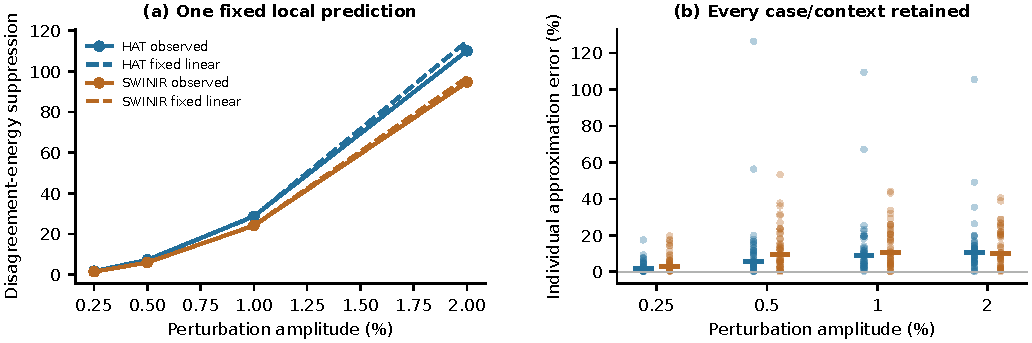
\includegraphics[width=.98\textwidth]{final_proposition_validation.pdf}
\caption{Fixed-context neural covariance experiment. (a) Mean observed coupled-minus-independent disagreement compared with the single .0025 odd-response prediction scaled by squared amplitude. (b) All individual relative approximation errors, including the 126.4\% boundary. The exact same-amplitude covariance closure is a separate identity check.}\label{fig:final-proposition}\end{figure*}

\subsection{Preserved historical headline figures}
These figures retain the original information contracts and estimands. They are not replaced numerically by the new acquired-only or cross-architecture results.
\begin{figure*}[t]\centering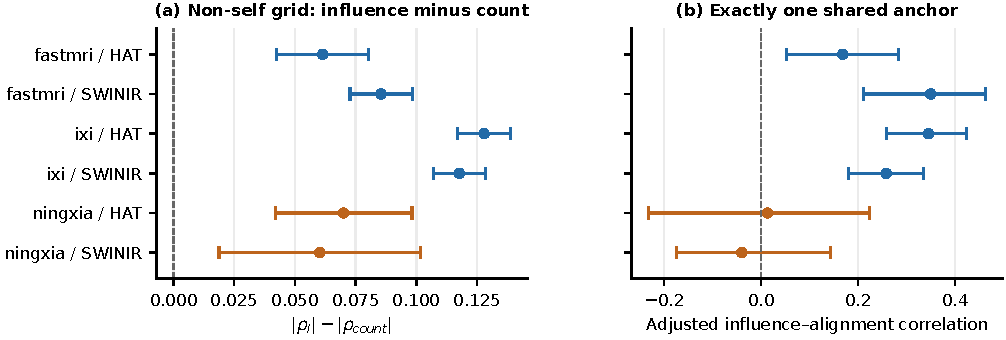
\includegraphics[width=.98\textwidth]{p17_influence_beyond_count.pdf}
\caption{Historical target-informed non-self influence advantage with six-stratum simultaneous intervals, alongside the fixed-count test with historical pointwise intervals. The NingXia null/mixed result remains.}\end{figure*}
\begin{table*}[t]\centering\small
\caption{Non-self broad grid and fixed-count influence. Broad-grid advantage uses six-stratum simultaneous 95\% intervals; fixed-count estimates retain historical pointwise clustered 95\% intervals. Both analyses preserve every cohort/model.}\label{tab:neural}
\begin{tabular}{llrrrr}\toprule
Cohort & Model & $\rho_{count}$ & $\rho_I$ & Non-self advantage [CI] & Fixed-one partial $\rho$ [CI]\\\midrule
fastmri & HAT & 0.704 & 0.766 & 0.061 [0.042,0.080] & 0.169 [0.053,0.283]\\
fastmri & SWINIR & 0.699 & 0.784 & 0.085 [0.073,0.098] & 0.350 [0.212,0.464]\\
ixi & HAT & 0.577 & 0.705 & 0.128 [0.117,0.139] & 0.346 [0.259,0.424]\\
ixi & SWINIR & 0.573 & 0.691 & 0.118 [0.107,0.128] & 0.258 [0.181,0.335]\\
ningxia & HAT & 0.620 & 0.690 & 0.070 [0.042,0.098] & 0.014 [-0.232,0.223]\\
ningxia & SWINIR & 0.609 & 0.669 & 0.060 [0.019,0.102] & -0.039 [-0.175,0.144]\\
\bottomrule\end{tabular}\end{table*}
\begin{figure*}[t]\centering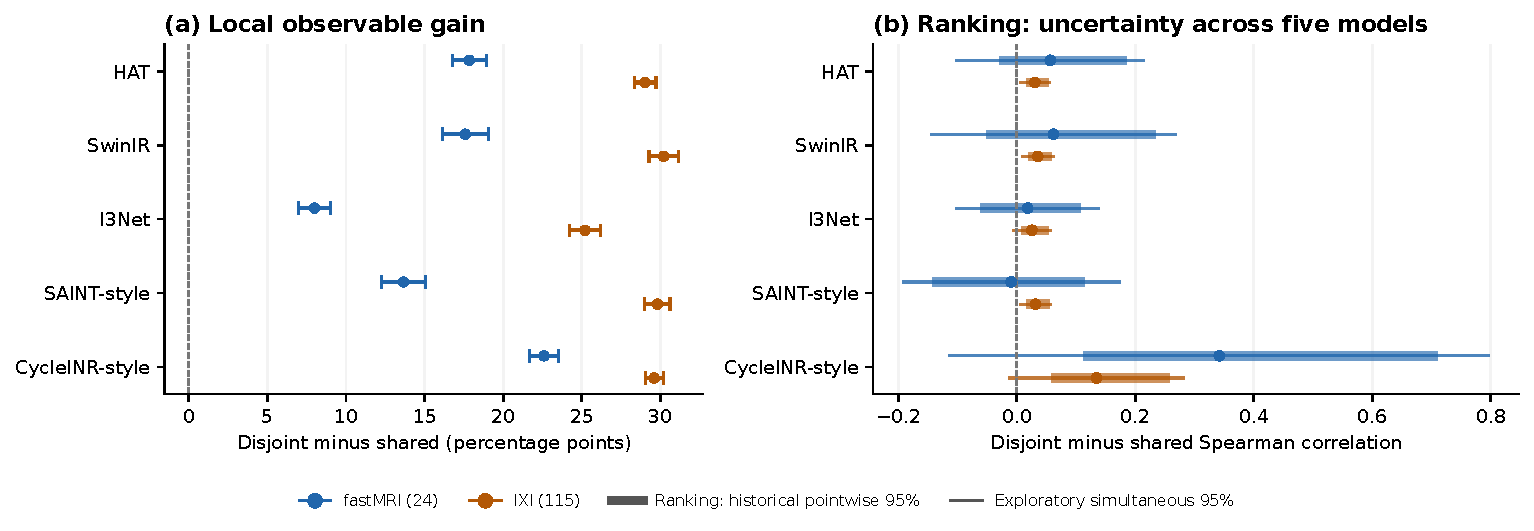
\includegraphics[width=.98\textwidth]{p13_architecture_robustness.pdf}
\caption{Historical same-model TTA replication: local effects versus examination ranking. Local fastMRI points use means and IXI medians; ranking uses within-examination medians. Five-model simultaneous intervals preserve the weak/null ranking results. Legacy SAINT coordinates are retained in this historical figure.}\end{figure*}

\subsection{A Practical Two-Member Ensemble Sharing Contrast}
We additionally evaluate fixed linear and four-point Lagrange cubic interpolators on IXI. Pairs L$_0$--C$_0$ versus L$_0$--C$_2$, and C$_0$--L$_0$ versus C$_0$--L$_2$, preserve target and estimator composition while varying the companion phase. The score support comes from phase-0 acquired anchors. Complete four-point support is required in both phases, with residue-1/3 equal weighting within cases. In 16-slice fastMRI, only $z=7$ meets both support requirements, not both residue classes: all 24 cases are excluded by that geometric rule. The initial eligibility assertion and correction of the protocol's mistaken expected target count are logged before proxy summaries; no boundary anchor is fabricated.

\begin{table*}[t]\centering\small
\caption{IXI two-member analytical ensemble, 115 examinations. Contrasts are disjoint minus shared, with simultaneous intervals over the two directions for each displayed endpoint. ``Fixed uses the unchanged reference predictor; ``paired uses both predictions.}
\begin{tabular}{llrr}\toprule
Proxy / metric & Error endpoint & L$_0$ reference [95\% CI] & C$_0$ reference [95\% CI]\\\midrule
Observable gain & --- & 0.3213 [0.3166,0.3260] & 0.3212 [0.3165,0.3259]\\
MAE disagreement & Fixed & 0.0428 [0.0188,0.0668] & 0.0473 [0.0220,0.0727]\\
MAE disagreement & Paired & 0.0471 [0.0228,0.0714] & 0.0470 [0.0228,0.0712]\\
Population variance & Fixed & 0.0313 [0.0122,0.0503] & 0.0361 [0.0158,0.0564]\\
Population variance & Paired & 0.0354 [0.0158,0.0550] & 0.0356 [0.0159,0.0552]\\
\bottomrule\end{tabular}\end{table*}

Population two-member variance is $|A-B|^2/4$ per pixel, pooled on the common support. It and MAE disagreement are related constructions, not independent experiments. Against fixed reference-model error, variance ranking improves by .0313/.0361, and MAE-disagreement ranking by .0428/.0473. Two-direction simultaneous intervals are positive in this IXI analytic experiment. Paired-error endpoints have the same direction and are separately tabulated. The five-architecture shared control is the complementary deterministic two-view TTA construction. Neither result establishes failure or success of all trained ensembles, stochastic posterior samplers, or calibrated uncertainty systems.

\subsection{Material Moved from the Main Paper}
The full native baseline table and retrospective practical-consequence plot move here to keep the main paper centered on phenomenon, influence and falsification. All 13 methods and 111 configurations remain, as do 20 training-budget comparisons and every adverse result. The historical common-support table below is a different evaluation contract from the complete native master table.
\begin{table*}[t]
\caption{All 13 master-table baselines at $\times4$, independently recovered from original metrics. PSNR/SSIM are higher-is-better; MAE is lower-is-better. Full-plane evaluation excludes acquired planes. IXI/fastMRI average examinations; NingXia averages eight patient folds. These values do not replace the masked common-support reliability endpoints.}
\label{tab:p15-master}\centering\small\setlength{\tabcolsep}{3.7pt}
\begin{tabular}{lrrrrrrrrr}\toprule
&\multicolumn{3}{c}{IXI (115)}&\multicolumn{3}{c}{fastMRI (24)}&\multicolumn{3}{c}{NingXia (8 folds)}\\
Method&PSNR&SSIM&MAE&PSNR&SSIM&MAE&PSNR&SSIM&MAE\\\midrule
Linear & 26.17 & 0.853 & 29.28 & 19.11 & 0.597 & 78.81 & 22.73 & 0.675 & 103.21\\
Cubic & 25.71 & 0.842 & 31.13 & 17.97 & 0.533 & 91.93 & 21.65 & 0.618 & 119.41\\
ACVTT & 27.34 & 0.882 & 25.52 & 20.19 & 0.662 & 71.55 & 23.47 & 0.728 & 95.44\\
Res-SRDiff & 28.04 & 0.882 & 24.19 & 21.67 & 0.691 & 56.34 & 21.15 & 0.554 & 153.02\\
ArSSR & 27.25 & 0.877 & 25.55 & 20.31 & 0.657 & 65.99 & 23.16 & 0.709 & 96.49\\
CycleINR-style & 26.17 & 0.853 & 29.28 & 20.32 & 0.658 & 66.10 & 22.90 & 0.693 & 101.10\\
ResUNet & 27.46 & 0.881 & 25.24 & 22.25 & 0.737 & 53.57 & 23.38 & 0.721 & 97.04\\
Pix2Pix-GAN & 27.11 & 0.851 & 27.02 & 21.91 & 0.729 & 53.26 & 22.45 & 0.711 & 105.81\\
SwinIR & 28.65 & 0.900 & 22.46 & 22.36 & 0.749 & 50.87 & 23.95 & 0.752 & 85.97\\
SAINT-style & 28.67 & 0.897 & 22.84 & 23.26 & 0.770 & 46.44 & 23.84 & 0.742 & 89.41\\
I3Net & 31.31 & 0.928 & 17.53 & 24.01 & 0.792 & 41.01 & 23.49 & 0.721 & 93.57\\
HAT & 28.72 & 0.902 & 22.25 & 23.09 & 0.769 & 47.25 & 23.95 & 0.752 & 86.14\\
SMamba-UNet & 29.35 & 0.908 & 21.14 & 22.73 & 0.762 & 49.45 & 23.91 & 0.750 & 86.82\\
\bottomrule\end{tabular}
\par\smallskip\parbox{.98\textwidth}{\footnotesize Locally adapted implementations retain their recorded training budgets; the master uses extended HAT training on fastMRI. This is not an equal-compute leaderboard. Standard and longer-budget results are reported separately.}
\end{table*}

\begin{figure*}[t]
\centering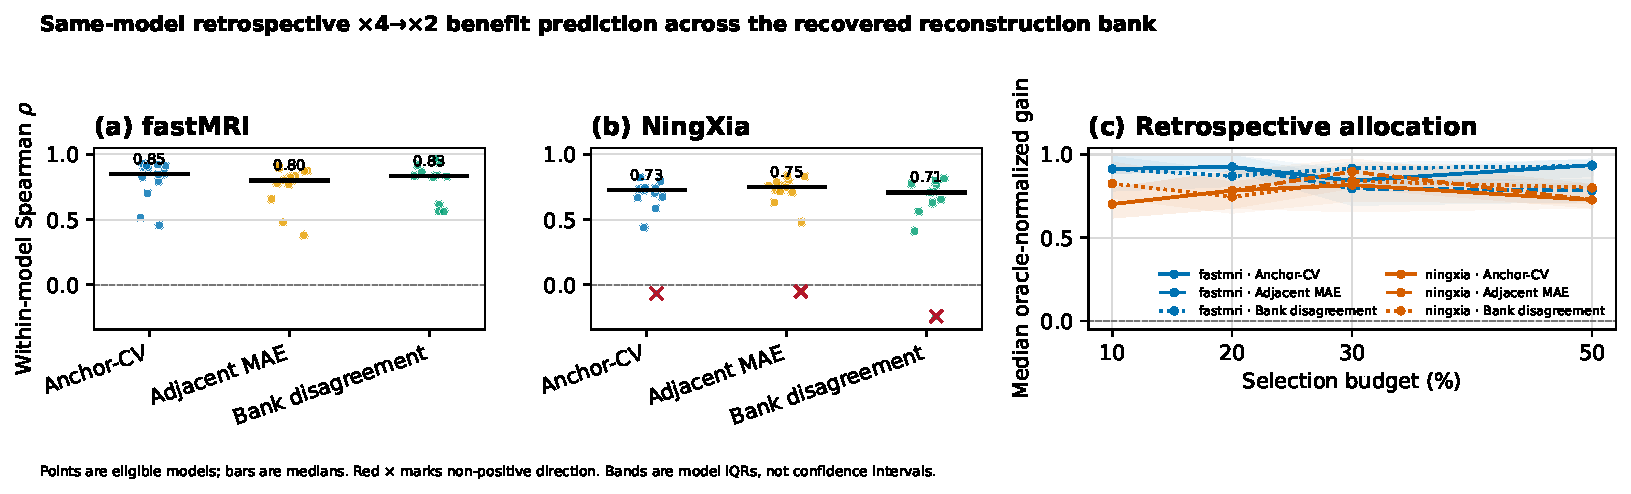
\includegraphics[width=.98\textwidth]{fig_same_model_consequence.pdf}
\caption{Fixed-rule retrospective same-model consequence, moved intact from the main paper. All eligible models remain; red crosses preserve adverse directions. Model-IQR bands are not confidence intervals. Factor-specific checkpoints can differ, and controlling current error weakens the benefit association.}
\label{fig:p17-moved-consequence}
\end{figure*}


\subsection{Exploratory Full-Model-Bank Audit}
After inspecting the recovered benchmark, we added an explicitly exploratory breadth audit; it is not part of the documented architecture-family test. On common case support within each cohort and factor, it covers 6--13 models, 483 undirected error pairs, and 807 directed target--member disagreement pairs. Independent bootstrap units are examinations for fastMRI/IXI and patient folds for NingXia.

Figure~\ref{fig:p10-bank} shows three results. First, median pairwise case-error rank correlation is .938/.963/.953 for fastMRI $\times2/\times4/\times6$, .991 for IXI $\times4$, and .992/.980/.972 for NingXia $\times2/\times4/\times6$. All seven clustered 95\% intervals have lower bounds above .83. Second, disagreement generally ranks target error, but target--member error dependence does not by itself determine that reliability. Third, a matched cross-family partner is better for several implicit targets yet neutral or worse for several transformer and attention-CNN targets; architecture family is not a universal selection rule.

The NingXia $\times2$ low tail is important rather than hidden: all 12 pairs with error-rank $\rho<.9$ contain the degraded Res-SRDiff run, whose MAE is 479.32 in the benchmark table. This outlier shows that a failed estimator may produce different errors without producing a generally useful reliability partner. We therefore report the full distribution and do not reinterpret independence as quality.

\begin{figure*}[t]
\centering
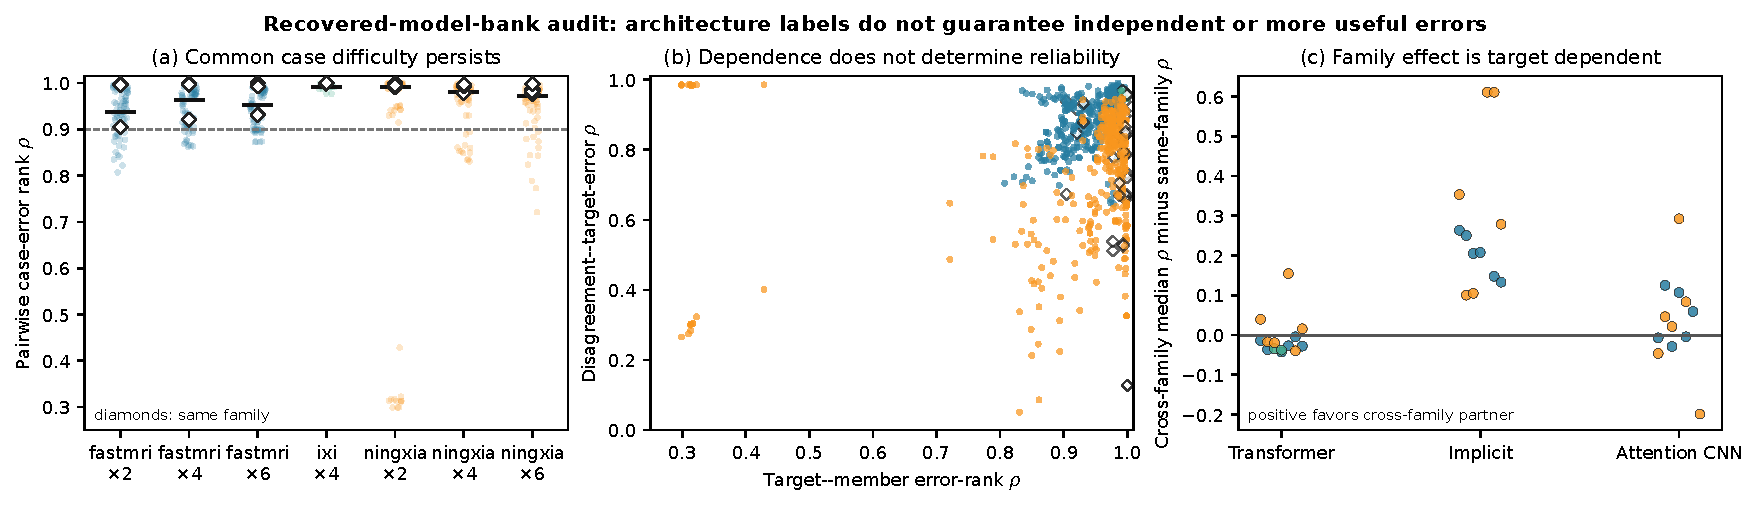
\includegraphics[width=.98\textwidth]{p10_model_bank_diversity.pdf}
\caption{Exploratory recovered-model-bank audit. (a) Case difficulty remains shared across architectures; diamonds denote same-family pairs. (b) Pairwise error dependence does not uniquely determine how disagreement ranks target error. (c) Cross-family minus matched same-family reliability can be positive or negative. Orange denotes NingXia, including the retained degraded Res-SRDiff boundary.}
\label{fig:p10-bank}
\end{figure*}

\begin{table*}[t]
\centering
\caption{Architecture-family same-target result on 24 fastMRI examinations at $\times4$. Observable gain is disjoint minus clean shared fraction. Ranking intervals resample examinations.}
\label{tab:p9-arch}
\setlength{\tabcolsep}{4pt}
\begin{tabular}{llrrr}
\toprule
Model & Family & Observable gain [95\% CI] & $\rho_{\rm shared}\rightarrow\rho_{\rm disjoint}$ & Ranking $\Delta\rho$ [95\% CI]\\
\midrule
HAT & Transformer SR & .178 [.170,.187] & .896$\rightarrow$.952 & .057 [$-.030$,.186]\\
SwinIR & Transformer SR & .176 [.164,.188] & .883$\rightarrow$.945 & .062 [$-.051$,.234]\\
I3Net & Inter/intra-slice CNN & .080 [.072,.088] & .943$\rightarrow$.961 & .018 [$-.061$,.107]\\
SAINT & Spatial conditional CNN & .137 [.125,.149] & .934$\rightarrow$.924 & $-.010$ [$-.143$,.114]\\
CycleINR & Implicit coordinate & .226 [.219,.233] & .634$\rightarrow$.976 & .342 [.113,.711]\\
\bottomrule
\end{tabular}
\end{table*}

The equal-weight four-family observable gain is .155 [.148,.162]. Leave-one-family-out estimates are .180 without I3Net, .131 without INR, .161 without SAINT, and .147 without transformers; all intervals exclude zero. The frozen shared-condition thresholds identify stable-wrong rates of 0 for HAT, SwinIR, I3Net, and SAINT and 4/120 (3.33\%) for CycleINR; CycleINR has 0/120 under disjoint contexts. This negative prevalence result is not replaced by the earlier earlier stable-wrong definition.

\subsection{Distinct-Cohort IXI Five-Architecture Replication}
The IXI architecture replication applies the same phase-0/phase-2 clean contrast to all 115 historically reused IXI reconstruction-test examinations, with five deterministic targets per examination and 5,000 examination-bootstrap replicates. The historical gate checked one IXI examination per wrapper. The final array audit additionally reproduces all 115 examinations per model with zero maximum absolute difference under the legacy mapping; new SAINT physical coordinates remain a separately declared correction. All five models, examinations, five targets and both conditions remain, without duplicate keys or non-finite metric values.

\begin{table*}[t]
\centering
\caption{Frozen IXI $\times4$ replication and reflection-matched identity swap. Effects are disjoint minus shared observable fraction. Clean and balanced effects are examination medians; mirror difference is residue-1 minus residue-3. All intervals resample examinations.}
\label{tab:p11-ixi-arch}
\setlength{\tabcolsep}{3.5pt}
\scriptsize
\begin{tabular}{lrrrr}
\toprule
Model & Clean gain [95\% CI] & Ranking $\Delta\rho$ [95\% CI] & Reflection-balanced gain [95\% CI] & Mirror difference [95\% CI] \\
\midrule
HAT & .290 [.286,.296] & .031 [.016,.053] & .292 [.286,.297] & .000 [$-.005$,.007] \\
SwinIR & .302 [.295,.307] & .035 [.019,.059] & .300 [.295,.308] & .001 [$-.003$,.006] \\
I3Net & .252 [.244,.260] & .025 [.008,.053] & .251 [.244,.257] & .002 [$-.004$,.012] \\
SAINT-style & .298 [.292,.305] & .032 [.017,.055] & .297 [.288,.302] & $-.0003$ [$-.006$,.006] \\
CycleINR-style & .296 [.291,.300] & .134 [.058,.258] & .295 [.290,.299] & .001 [$-.0004$,.004] \\
\bottomrule
\end{tabular}
\end{table*}

Every historical pointwise clean and reflection-balanced gain interval is positive, and every model has a positive effect in all 115 examinations. The clean equal-weight family estimate is .286; leave-one-family-out estimates are .281--.297. The signed mirror-difference interval includes zero for every model, so the frozen orientation-warning list is empty. This supports physical anchor identity after matching the nearest-distance multiset $\{1,3\}$ up to reflection. It does not establish exact signed-geometry identity, because the two residue classes are reflection-equivalent rather than identical.

\subsection{Controlled Dependence Results}
The original pooled-plane ranking and stable-wrong summaries are retained here without changing their endpoints, thresholds or weights. They differ from the uniform local-error estimand used by the revised main Figure 2 and Table 1.
\begin{figure*}[t]\centering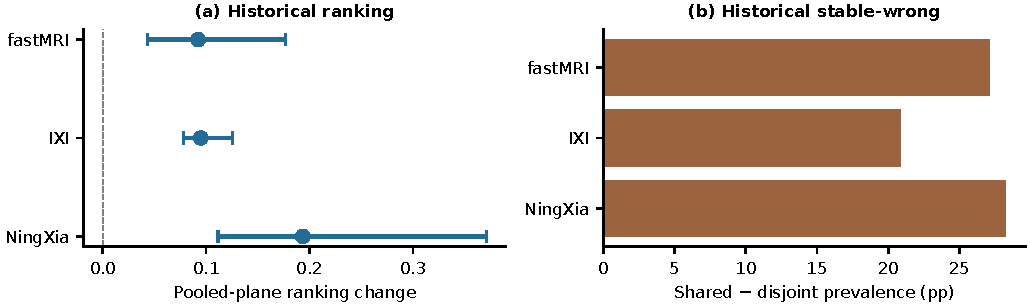
\includegraphics[width=.97\textwidth]{historical_ranking_prevalence.pdf}
\caption{Retained historical pooled-plane disagreement ranking and stable-wrong prevalence. Ranking uses fixed phase-0 MAE on fastMRI/NingXia and disjoint-pair MAE on IXI. Intervals resample examination/patient clusters; prevalence uses the original test-relative thresholds. Neither is an examination-level point correlation or calibrated event rate.}
\end{figure*}
\begin{table*}[t]
\centering
\caption{Original clean shared/disjoint comparison. Ranking against a fixed endpoint (phase-0 MAE on fastMRI/NingXia; disjoint-pair mean MAE on IXI) pools plane/model observations; intervals resample examinations/patients. Stable-wrong thresholds are test-relative, fixed from the disjoint condition.}
\label{tab:historical-controlled}
\setlength{\tabcolsep}{4pt}
\begin{tabular}{lrrrrr}
\toprule
Cohort & Independent units & $\rho_{\rm disjoint}$ & $\rho_{\rm shared}$ & $\Delta\rho$ [95\% CI] & Observable error / stable-wrong $\Delta$ \\
\midrule
fastMRI & 24 examinations & .959 & .867 & .092 [.043,.176] & 2.61\% / +27.1 pp \\
IXI & 115 examinations & .981 & .886 & .095 [.078,.126] & 1.58\% / +20.9 pp \\
NingXia & 8 patients (22 series) & .892 & .698 & .193 [.111,.371] & .25\% / +28.2 pp \\
\bottomrule
\end{tabular}
\end{table*}

\begin{table*}[t]
\centering
\caption{Clean same-target dependence control. Stable-wrong $\Delta$ uses high-error/low-disagreement thresholds frozen from the zero-overlap condition.}
\label{tab:clean-full}
\setlength{\tabcolsep}{4pt}
\begin{tabular}{lrrrrr}
\toprule
Cohort & Units & $\rho_{\rm disjoint}$ & $\rho_{\rm shared}$ & $\Delta\rho$ [95\% CI] & Shared / observable error \\
\midrule
fastMRI & 24 examinations & .959 & .867 & .092 [.043,.176] & 97.39\% / 2.61\% \\
IXI & 115 examinations & .981 & .886 & .095 [.078,.126] & 98.42\% / 1.58\% \\
NingXia & 8 patients, 22 series & .892 & .698 & .193 [.111,.371] & 99.75\% / .25\% \\
\bottomrule
\end{tabular}
\end{table*}

The original order-reversal control is not used as the cleaner dependence contrast. It supports the complete covariance chain on IXI and NingXia, but several cosine/shared/observable arrows reverse on fastMRI because order reversal changes more than anchor dependence. The horizontal-flip clean control preserves anchor identities, target, distances, count, $z$ order, mask, and preprocessing and is the cleaner historical TTA intervention. The final cross-architecture primary experiment uses no TTA.

Metric robustness was assessed over MAE, RMSE/MSE, SSIM error, gradient MAE, low-pass MAE, and residual high-frequency MAE for three physical planes, three cohorts, and two architectures. All 42 disjoint-minus-shared point differences are positive. All seven IXI intervals exclude zero. SSIM error has weak or negative absolute ranking on fastMRI/NingXia and several smaller-cohort gradient/high-frequency intervals cross zero. The claim is broad error observability, not metric independence.

\subsection{Exact Count Falsification and Analytical Influence}
The compact analytical ladder uses all valid sign configurations at fixed absolute distances $\{1,2,3,4\}$. Across fastMRI, IXI, and NingXia, overlap count has overall $+.9$ association with error cosine/shared fraction and $-.9$ to $-1.0$ with observable fraction/disagreement. Every cohort nevertheless shows a zero-to-one reversal. A wider $\{2,4,6,8\}$ ladder reproduces the exception on IXI while NingXia is monotone. This rejects strict count monotonicity without rejecting a broad dependence effect.

\begin{table*}[t]
\centering
\caption{Analytical shared influence versus count. Values are Spearman association with error alignment.}
\label{tab:analytic}
\setlength{\tabcolsep}{5pt}
\begin{tabular}{lrrr}
\toprule
Cohort & Count & Common coefficient mass & Gain \\
\midrule
fastMRI & .503 & .815 & .312 \\
IXI & .466 & .789 & .323 \\
NingXia & .630 & .855 & .225 \\
\bottomrule
\end{tabular}
\end{table*}

For the four main analytical endpoints, clustered intervals for the absolute-correlation improvement of common coefficient mass over count are all above zero, spanning .189--.283. Signed dot product and coefficient cosine agree qualitatively; common mass is reported because it retains unequal shared magnitude.

\subsection{Full Neural Shared-Influence Results}
\begin{table*}[t]
\centering
\caption{Broad neural context grid. $\rho_c$ uses overlap count and $\rho_I$ neural shared influence. Advantage intervals are clustered.}
\label{tab:neural-full}
\scriptsize
\setlength{\tabcolsep}{3pt}
\begin{tabular}{llrrrrrr}
\toprule
Cohort & Model & $\rho_c$ align. & $\rho_I$ align. & Adv. [95\% CI] & $\rho_I$ shared & $\rho_I$ observable & partial $\rho_I$ align. \\
\midrule
fastMRI & HAT & .799 & .838 & .039 [.028,.049] & .829 & $-.830$ & .359 \\
 & SwinIR & .796 & .851 & .055 [.048,.061] & .845 & $-.845$ & .395 \\
IXI & HAT & .714 & .797 & .082 [.076,.088] & .794 & $-.795$ & .315 \\
 & SwinIR & .712 & .787 & .075 [.070,.080] & .786 & $-.787$ & .289 \\
NingXia & HAT & .743 & .786 & .043 [.027,.057] & .792 & $-.792$ & .235 \\
 & SwinIR & .735 & .772 & .036 [.016,.057] & .781 & $-.781$ & .197 \\
\bottomrule
\end{tabular}
\end{table*}

The corresponding primary shared-fraction and observable-fraction advantages are .040/.040 and .056/.056 on fastMRI, .089/.089 and .081/.081 on IXI, and .049/.049 and .043/.043 on NingXia for HAT/SwinIR. Every interval excludes zero. Direct disagreement improves in all six strata, but both fastMRI intervals cross zero; it is supporting rather than primary evidence.

\subsubsection{Fixed-one-overlap test}
\begin{table*}[t]
\centering
\caption{Neural influence partial Spearman at exactly one shared anchor, controlling span, asymmetry, and examination. Error-alignment intervals are shown.}
\label{tab:fixed}
\setlength{\tabcolsep}{4pt}
\begin{tabular}{llrrrr}
\toprule
Cohort & Model & Error alignment & Shared fraction & Observable fraction & Disagreement \\
\midrule
fastMRI & HAT & .169 [.053,.283] & .135 & $-.135$ & $-.161$ \\
 & SwinIR & .350 [.212,.464] & .321 & $-.321$ & $-.286$ \\
IXI & HAT & .346 [.259,.424] & .360 & $-.360$ & $-.543$ \\
 & SwinIR & .258 [.181,.335] & .241 & $-.241$ & $-.587$ \\
NingXia & HAT & .014 [$-.232$,.223] & $-.006$ & .006 & $-.102$ \\
 & SwinIR & $-.039$ [$-.175$,.144] & $-.039$ & .039 & $-.072$ \\
\bottomrule
\end{tabular}
\end{table*}

NingXia does not preserve the expected direction consistently and all intervals cross zero. We therefore do not use wording such as “the direction is preserved but less precise.” The actual result is null/mixed under eight-patient fixed-count inference.

\subsubsection{Perturbation and plane stability}
The perturbation-stability audit varies amplitude (.5/1/2\%), positive/negative field, Rademacher/Gaussian field, and 1/2/4/8 directions. All 42 cohort--architecture--condition strata pass the frozen rank-stability threshold; minimum Spearman is .942 and maximum .999. Physical-plane pair stability is .779--.954, and only one of three plane-pair gates passes. This makes the statistic robust to the tested numerical perturbation design but local to a declared physical plane.

\subsection{Mechanism Chain}
\begin{table*}[t]
\centering
\caption{Partial Spearman ranges across HAT/SwinIR. Local arrows are supported in every stratum. “Ranking” counts architecture intervals excluding zero.}
\label{tab:chain}
\setlength{\tabcolsep}{3.5pt}
\begin{tabular}{lrrrr}
\toprule
Cohort & Influence$\rightarrow$alignment & Alignment$\rightarrow$norm. disagreement & Influence$\rightarrow$observable & Alignment$\rightarrow$ranking \\
\midrule
fastMRI & .372--.410 & $-.933$--$-.926$ & $-.412$--$-.370$ & $-.333$--$-.143$ (0/2) \\
IXI & .321--.347 & $-.893$--$-.890$ & $-.342$--$-.298$ & $-.643$--$-.500$ (2/2) \\
NingXia & .219--.258 & $-.898$--$-.889$ & $-.231$--$-.211$ & $-.667$--$-.548$ (1/2) \\
\bottomrule
\end{tabular}
\end{table*}

The context-ranking endpoint uses only eight configurations and is not a mediation estimate. Influence-to-ranking is still less stable. The manuscript therefore claims that influence is one determinant of local error alignment/observability, not that it alone determines global case ranking.

\subsection{Anchor-CV, Strong Baselines, and Consequence}
Anchor-CV exactly equals the masked MAE of half the acquired-slice second difference. Frozen-score reproduction has maximum absolute error $5.68\times10^{-14}$. Table~\ref{tab:anchor} reports strong baselines that prevent a uniqueness claim.

\begin{table*}[t]
\centering
\caption{Examination-level $\times4$ difficulty ranking. Lower nAURC is better.}
\label{tab:anchor}
\setlength{\tabcolsep}{5pt}
\begin{tabular}{llrrr}
\toprule
Cohort & Method & Spearman & Kendall & nAURC \\
\midrule
fastMRI & Anchor-CV / adjacent MAE / adjacent RMSE & .943 / .934 / .942 & .812 / .790 / .804 & .0231 / .0222 / .0241 \\
IXI & Anchor-CV / adjacent MAE / adjacent RMSE & .955 / .956 / .956 & .831 / .834 / .826 & .0150 / .0145 / .0147 \\
NingXia & Anchor-CV / adjacent MAE / adjacent RMSE & .958 / .973 / .959 & .844 / .879 / .835 & .0112 / .0072 / .0123 \\
\bottomrule
\end{tabular}
\end{table*}

Partial rank association for Anchor-CV after adjacent MAE, robust scale, and spacing is .333 on fastMRI, $-.059$ on IXI, and $-.100$ on NingXia. Scale normalization reduces/reverses rankings, so the score is not a scale-free invariant. Frozen risk--coverage also has no universal winner: output PC is better on fastMRI/IXI and adjacent MAE is better on NingXia.

The fixed-rule retrospective consequence audit instead matches model identity while allowing factor-specific weights. It pairs common-support $\times4$ and $\times2$ MAE for every eligible model on fastMRI and patient-folded NingXia. Anchor-CV is positively associated with benefit for 13/13 fastMRI models and 12/13 NingXia models (median within-model $\rho=.851/.727$); adjacent MAE gives 13/13 and 12/13 (.802/.748), and candidate-bank disagreement gives 11/11 and 10/11 (.835/.710). The smaller bank denominator is structural: the precomputation includes neural targets only; Linear/Cubic are candidate members but not target rows. The only non-positive model is the severely degraded NingXia Res-SRDiff run; all three intervals cross zero. No model is removed by result direction.

At 10/20/30/50\% selection budgets, model-median oracle-normalized gains remain positive for all three scores in both cohorts. Individual NingXia Res-SRDiff policies can fall below random, so allocation is not universally beneficial. These analyses use already reconstructed dense acquisitions and cannot identify the causal scanner-time benefit of changing acquisition density.

Anchor-CV takes .42/3.97/3.93 ms CPU on representative fastMRI/IXI/NingXia examinations with zero neural calls. Output PC is cheap only after predictions exist. Neither Anchor-CV nor PC localizes the worst physical plane; their supported use is examination triage.

\subsection{Exploratory Robustness and Information Audit}
These analyses were designed after inspecting existing results. They add no independent cohort and are not prospectively registered. All five architectures, both brain cohorts, all eligible benefit models, and adverse outcomes are retained. Bootstrap count is 10,000; the seed is 20260908.

\paragraph{Aggregation and simultaneous inference.}
We recompute observable gain with all four combinations of within-case and across-case mean/median aggregation. Every model retains a positive five-model simultaneous interval in every combination and cohort. Intervals use the maximum absolute bootstrap deviation divided by each estimate's bootstrap standard deviation, with shared examination draws across models. They are approximate bootstrap simultaneous intervals, not exact small-sample coverage guarantees. Historical fastMRI local gain uses mean/mean aggregation, whereas ranking uses within-case medians; IXI uses medians. Cohorts remain separate.

The more fragile endpoint is ranking. Under historical within-case median aggregation, simultaneous intervals exclude zero for IXI HAT, SwinIR and SAINT only; I3Net and CycleINR include zero. No fastMRI ranking interval excludes zero under simultaneous inference, including CycleINR. Historical pointwise intervals remain reported; they answer a different multiplicity question. Averaging the two conditions' paired errors to obtain a common ranking endpoint gives the same three-versus-zero simultaneous pattern. This common endpoint remains post-intervention and is not a fixed phase-0 error estimate.

\paragraph{Densification and current-error coupling.}
For the existing 598 rows, $b=E_4-E_2$ is checked exactly and models are paired on the same case, fold and support. Matching labels does not hold scale-specific checkpoints fixed. Since $b$ contains $E_4$, raw score--benefit association need not establish incremental information beyond current difficulty. We regress ranks of score and benefit on the rank of $E_4$ and correlate residuals, reranking within each bootstrap sample. NingXia resamples eight patients with subordinate series retained; degenerate partial-correlation replicates are recorded rather than silently counted as zero.

\begin{table*}[t]
\centering\small
\caption{Current-error sensitivity, with every eligible model retained. Entries are model-median correlations; the final column counts positive pointwise partial-correlation intervals. This is a diagnostic adjustment using retrospective target error, not a deployable score.}
\begin{tabular}{llrrr}
\toprule
Cohort&Score&Raw $\rho$&Partial $\rho\mid E_4$&Positive partial CI / models\\
\midrule
fastMRI&Anchor-CV&.851&.203&0/13\\
&Adjacent MAE&.802&$-.068$&0/13\\
&Bank disagreement&.835&.056&1/11\\
NingXia&Anchor-CV&.727&.291&0/13\\
&Adjacent MAE&.748&.426&1/13\\
&Bank disagreement&.710&.389&0/11\\
\bottomrule
\end{tabular}
\end{table*}

\begin{figure*}[t]
\centering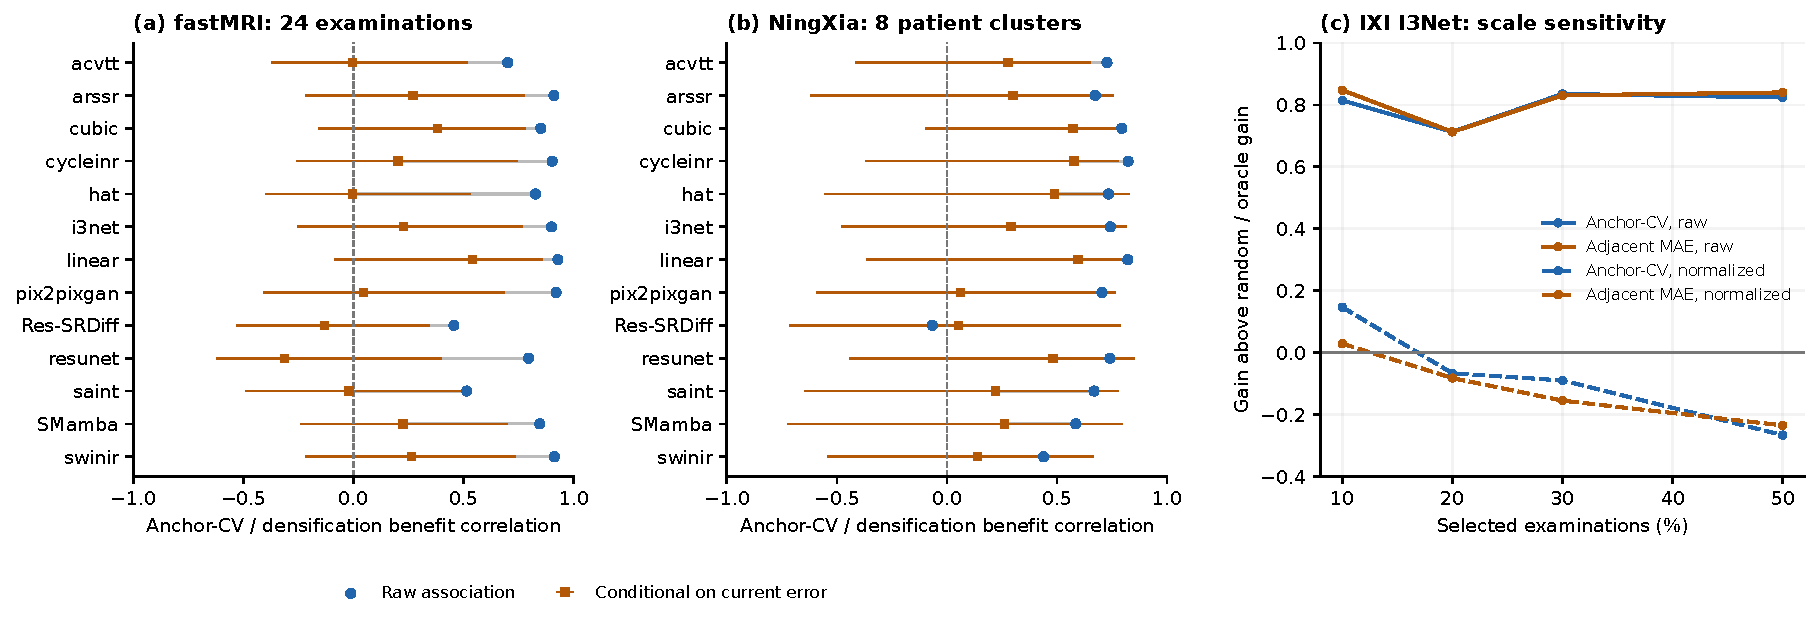
\includegraphics[width=\textwidth]{p13_benefit_boundaries.pdf}
\caption{Benefit boundaries. (a,b) Raw Anchor-CV associations (blue) and associations conditional on current error (orange), with patient/examination-bootstrap 95\% intervals for the latter. All 26 conditional intervals cross zero. (c) Recovered IXI I3Net allocation shows a reversal after acquired-range normalization against the same raw-scale benefit endpoint. Lines are point estimates, not uncertainty bands.}
\label{fig:p13-benefit}
\end{figure*}

\paragraph{Recovered IXI same-architecture pair.}
The existing I3Net $\times2$ and $\times4$ profiles each contain 115 outputs and distinct checkpoints. All 7,334 common odd target planes are re-evaluated with identical physical affines and a common target-derived 1\% mask; case MAE averages planes before inference. Mean MAE is 33.65 at $\times4$ and 25.62 at $\times2$, with positive benefit for 115/115 examinations. Linear interpolation on this support gives 57.36 and 39.21. These numbers are not interchangeable with the benchmark's all-generated-plane averages.

Anchor-CV and adjacent MAE, computed only from $\times4$ acquired anchors, give raw benefit correlations .843 [.768,.894] and .845 [.771,.896]. Their partial correlations given current error are .216 [.007,.430] and .227 [.020,.437]. These exploratory pointwise intervals do not imply universal superiority. Dividing the scores by the acquired-anchor 1st--99th percentile range reverses raw-benefit ranking to $-.238$ [$-.404,-.058$] and $-.236$ [$-.397,-.060$]. At 50\% selection normalized Anchor-CV is below random by .920 raw MAE units [$-1.635,-.149$]. The endpoint is deliberately left in raw units: this establishes sensitivity to the scoring scale, not failure of every jointly normalized evaluation.

\paragraph{Algebra and information access.}
Writing $T$ for mean paired squared error and $q$ for shared fraction, normalized RMSE disagreement equals $2\sqrt{1-q}$. The historical TMI script actually uses MAE disagreement, so its statistic is $2\kappa\sqrt{1-q}$ with $\kappa=\mathrm{MAE}(a-b)/\mathrm{RMSE}(a-b)\leq1$. The residual-shape factor must not be omitted. The shared-fraction correlation is structurally coupled and does not independently establish a mechanism.

The historical architecture studies output-score mask uses dense targets. The bank instead uses target-model prediction support; its field name does not denote ground truth. Raw Anchor-CV and adjacent MAE use acquired-only masks. The earlier scale-normalized Anchor-CV uses a full-volume robust range, whereas the new IXI normalization explicitly uses acquired anchors. Deployment requires a separately frozen acquisition-only mask and scale convention. Exact wrapper agreement validates implementation consistency for the tested cases, not freedom from target-support bias or general model correctness.

\paragraph{Reproducibility.}
The new scripts, source hashes, geometry checks, complete model-specific intervals, leave-one-cluster-out tables and patient-equal sensitivity results are retained in the final reproducibility and evidence map. All reported values are regenerated from the formal CSV records; technical smoke outputs are excluded by declared file identity.


\subsection{Complete Baseline Ledger and Training-Budget Sensitivity}
The experiment master table contains 13 reconstruction baselines. We recover all 39 three-cohort $\times4$ rows, all 52 fastMRI/NingXia $\times2/\times6$ rows, and all 20 recorded longer-budget rows: 111 configurations and 555 metric values. Original metric summaries agree to their reported four-decimal precision. Two overwritten SAINT summaries at fastMRI $\times2/\times6$ are recovered from all 48 preserved output volumes. No run is retrained for this audit.

The native evaluator measures every nonacquired plane on the whole image, averages planes within an examination, and then averages examinations. NingXia first averages series within a held-out patient fold, then averages all eight folds. PSNR uses each target plane's range; SSIM is the full-plane implementation. These are reference-based evaluation metrics, not deployable QA scores. Each configuration has matching case identities and generated-plane counts across its models; this count audit does not independently certify all historical preprocessing. The old masked common-support tables and this native-metric ledger remain distinct contracts. Automatic threshold-mask Dice/HD95 columns are not interpreted as anatomical segmentation.

All model names denote the local implementations, including generic SR models adapted to 2.5-D conditioning, inherited GAN, and local SAINT/CycleINR variants. The recorded master profiles include different training budgets and early stopping; no equal-compute claim is made. PAST-Net's fastMRI development trajectory remains development evidence rather than a new independent three-cohort baseline result.

\paragraph{What the full bank adds.}
Using all 13 native-metric baselines gives 78 model pairs per cohort. Median case-error rank correlations are .997 on IXI, .899 on fastMRI, and 1.000 on eight NingXia patient folds. These descriptive estimates show shared difficulty across the full bank while retaining the lower fastMRI association than in the masked analysis. They do not imply independent model pairs or extend the five-model intervention to 13 models.

\paragraph{Budget protocol and negative boundaries.}
For every recorded 60/90-epoch experiment, compare its matched standard-profile cases; use 10,000 paired bootstrap draws (seed 20260910), examinations for fastMRI and patient folds for NingXia. The primary MAE intervals simultaneously cover all 20 comparisons using the bootstrap maximum standardized deviation. All five metric changes remain in the numerical record. Fifteen MAE intervals favor longer training; five cross zero. Runs are separate training experiments, not a controlled single-checkpoint continuation, and standard values are never replaced by their best budget.

NingXia Res-SRDiff $\times2$ MAE changes from 440.61 at 30 epochs to 140.45 at 60 and 118.25 at 90, still above Linear's 78.53. A short-budget failure therefore cannot establish an intrinsic diffusion-family failure. Conversely, CycleINR $\times2$ barely changes (.000006 MAE reduction), and five simultaneous intervals remain inconclusive. The source note that fastMRI ACVTT $\times6$ worsened at 60 epochs is contradicted by its numbers: PSNR improves 19.8309 to 20.0269, and MAE 72.4367 to 70.9050; all five metric directions improve. The original note is preserved and this correction is explicit.
\begin{table*}[t]\centering\small
\caption{IXI $\times4$: complete native metrics, recorded master profile.}
\begin{tabular}{lrrrrr}\toprule Method&PSNR&SSIM&MAE&MSE&NCC\\\midrule
Linear & 26.1722 & 0.8529 & 29.2781 & 6553.8673 & 0.9390\\
Cubic & 25.7138 & 0.8422 & 31.1269 & 7217.2979 & 0.9303\\
ACVTT & 27.3431 & 0.8822 & 25.5217 & 5206.8325 & 0.9557\\
Res-SRDiff & 28.0441 & 0.8821 & 24.1938 & 4664.4129 & 0.9611\\
ArSSR & 27.2467 & 0.8773 & 25.5509 & 5267.3658 & 0.9533\\
CycleINR-style & 26.1728 & 0.8527 & 29.2765 & 6553.8469 & 0.9390\\
ResUNet & 27.4611 & 0.8812 & 25.2395 & 4985.4989 & 0.9552\\
Pix2Pix-GAN & 27.1070 & 0.8506 & 27.0202 & 5372.2668 & 0.9538\\
SwinIR & 28.6485 & 0.8997 & 22.4556 & 4137.5109 & 0.9658\\
SAINT-style & 28.6677 & 0.8970 & 22.8365 & 4128.0151 & 0.9660\\
I3Net & 31.3058 & 0.9285 & 17.5276 & 2565.3177 & 0.9788\\
HAT & 28.7249 & 0.9016 & 22.2500 & 4088.7422 & 0.9663\\
SMamba-UNet & 29.3536 & 0.9077 & 21.1352 & 3691.2381 & 0.9699\\
\bottomrule\end{tabular}\end{table*}
\begin{table*}[t]\centering\small
\caption{fastMRI $\times4$: complete native metrics, recorded master profile.}
\begin{tabular}{lrrrrr}\toprule Method&PSNR&SSIM&MAE&MSE&NCC\\\midrule
Linear & 19.1133 & 0.5970 & 78.8111 & 23092.0046 & 0.7733\\
Cubic & 17.9736 & 0.5332 & 91.9330 & 29740.2642 & 0.7285\\
ACVTT & 20.1941 & 0.6624 & 71.5480 & 18286.6190 & 0.8320\\
Res-SRDiff & 21.6727 & 0.6909 & 56.3371 & 13095.4191 & 0.8814\\
ArSSR & 20.3143 & 0.6575 & 65.9931 & 17745.8948 & 0.8301\\
CycleINR-style & 20.3156 & 0.6577 & 66.0985 & 17743.2358 & 0.8302\\
ResUNet & 22.2549 & 0.7374 & 53.5705 & 11842.8147 & 0.8955\\
Pix2Pix-GAN & 21.9090 & 0.7294 & 53.2622 & 12485.1668 & 0.8915\\
SwinIR & 22.3578 & 0.7494 & 50.8733 & 11636.3791 & 0.8977\\
SAINT-style & 23.2605 & 0.7705 & 46.4417 & 9347.6662 & 0.9177\\
I3Net & 24.0102 & 0.7921 & 41.0101 & 7755.6546 & 0.9308\\
HAT & 23.0894 & 0.7688 & 47.2467 & 9773.1765 & 0.9138\\
SMamba-UNet & 22.7322 & 0.7618 & 49.4487 & 10826.4468 & 0.9051\\
\bottomrule\end{tabular}\end{table*}
\begin{table*}[t]\centering\small
\caption{NingXia $\times4$: complete native metrics, recorded master profile.}
\begin{tabular}{lrrrrr}\toprule Method&PSNR&SSIM&MAE&MSE&NCC\\\midrule
Linear & 22.7335 & 0.6749 & 103.2052 & 42189.1127 & 0.8576\\
Cubic & 21.6460 & 0.6184 & 119.4078 & 53313.5368 & 0.8252\\
ACVTT & 23.4735 & 0.7281 & 95.4376 & 35779.4840 & 0.8804\\
Res-SRDiff & 21.1538 & 0.5538 & 153.0213 & 66533.1526 & 0.8207\\
ArSSR & 23.1634 & 0.7091 & 96.4890 & 38343.9409 & 0.8708\\
CycleINR-style & 22.9009 & 0.6935 & 101.0990 & 40735.3568 & 0.8625\\
ResUNet & 23.3816 & 0.7209 & 97.0409 & 36316.2290 & 0.8785\\
Pix2Pix-GAN & 22.4530 & 0.7112 & 105.8119 & 46398.6707 & 0.8552\\
SwinIR & 23.9513 & 0.7525 & 85.9679 & 32030.5455 & 0.8930\\
SAINT-style & 23.8350 & 0.7422 & 89.4140 & 32992.9496 & 0.8905\\
I3Net & 23.4911 & 0.7208 & 93.5655 & 35725.4805 & 0.8825\\
HAT & 23.9499 & 0.7519 & 86.1449 & 32226.9860 & 0.8933\\
SMamba-UNet & 23.9126 & 0.7500 & 86.8152 & 32498.3175 & 0.8917\\
\bottomrule\end{tabular}\end{table*}
\begin{table*}[t]\centering\small
\caption{fastMRI $\times2$: complete native metrics, recorded master profile.}
\begin{tabular}{lrrrrr}\toprule Method&PSNR&SSIM&MAE&MSE&NCC\\\midrule
Linear & 21.6348 & 0.7030 & 53.9754 & 11591.9388 & 0.8732\\
Cubic & 20.3321 & 0.6363 & 64.1081 & 15236.6373 & 0.8370\\
ACVTT & 21.7910 & 0.7110 & 53.4000 & 11160.0709 & 0.8783\\
Res-SRDiff & 22.4766 & 0.6511 & 50.3378 & 9901.7857 & 0.9034\\
ArSSR & 23.1137 & 0.7613 & 43.5812 & 8391.3334 & 0.9140\\
CycleINR-style & 23.0957 & 0.7593 & 43.7063 & 8411.5115 & 0.9132\\
ResUNet & 24.1700 & 0.7913 & 39.7905 & 6909.6572 & 0.9338\\
Pix2Pix-GAN & 26.0734 & 0.8302 & 31.2304 & 4584.5238 & 0.9565\\
SwinIR & 24.8716 & 0.8153 & 35.9392 & 5990.3711 & 0.9428\\
SAINT-style & 24.4308 & 0.7809 & 39.6861 & 6749.7212 & 0.9373\\
I3Net & 27.7711 & 0.8670 & 25.3325 & 3113.5377 & 0.9700\\
HAT & 24.6475 & 0.8106 & 37.2729 & 6225.7429 & 0.9409\\
SMamba-UNet & 24.6548 & 0.8077 & 37.1110 & 6361.0863 & 0.9401\\
\bottomrule\end{tabular}\end{table*}
\begin{table*}[t]\centering\small
\caption{fastMRI $\times6$: complete native metrics, recorded master profile.}
\begin{tabular}{lrrrrr}\toprule Method&PSNR&SSIM&MAE&MSE&NCC\\\midrule
Linear & 18.2648 & 0.5595 & 88.2647 & 28258.4309 & 0.7215\\
Cubic & 18.2648 & 0.5595 & 88.2647 & 28258.4309 & 0.7215\\
ACVTT & 19.8309 & 0.6601 & 72.4367 & 20031.3896 & 0.8120\\
Res-SRDiff & 21.2529 & 0.6791 & 59.4388 & 14747.2531 & 0.8702\\
ArSSR & 19.4214 & 0.6156 & 74.9270 & 21914.5364 & 0.7872\\
CycleINR-style & 19.3873 & 0.6158 & 74.9017 & 22086.6021 & 0.7854\\
ResUNet & 22.1434 & 0.7375 & 53.8609 & 12277.0333 & 0.8921\\
Pix2Pix-GAN & 21.6510 & 0.7250 & 54.8359 & 13567.5373 & 0.8828\\
SwinIR & 21.8398 & 0.7305 & 56.4490 & 13267.8010 & 0.8840\\
SAINT-style & 22.3172 & 0.7466 & 52.5303 & 11683.3596 & 0.8979\\
I3Net & 22.8308 & 0.7617 & 47.0732 & 10309.8900 & 0.9088\\
HAT & 21.8230 & 0.7313 & 55.7775 & 13341.4608 & 0.8829\\
SMamba-UNet & 21.9153 & 0.7313 & 56.5002 & 13166.6662 & 0.8848\\
\bottomrule\end{tabular}\end{table*}
\begin{table*}[t]\centering\small
\caption{NingXia $\times2$: complete native metrics, recorded master profile.}
\begin{tabular}{lrrrrr}\toprule Method&PSNR&SSIM&MAE&MSE&NCC\\\midrule
Linear & 24.9741 & 0.7264 & 78.5349 & 27551.4768 & 0.9112\\
Cubic & 24.1081 & 0.6767 & 89.5215 & 33708.1987 & 0.8952\\
ACVTT & 25.3139 & 0.7518 & 76.2396 & 25631.8031 & 0.9180\\
Res-SRDiff & 15.3187 & 0.2945 & 440.6059 & 311894.3839 & 0.8320\\
ArSSR & 25.1538 & 0.7427 & 76.6719 & 26571.4634 & 0.9146\\
CycleINR-style & 25.1538 & 0.7427 & 76.6723 & 26571.4525 & 0.9146\\
ResUNet & 25.2629 & 0.7478 & 76.6937 & 25684.3115 & 0.9170\\
Pix2Pix-GAN & 25.2116 & 0.7543 & 74.8168 & 25448.9329 & 0.9169\\
SwinIR & 25.5845 & 0.7651 & 73.1350 & 24249.0709 & 0.9226\\
SAINT-style & 25.3398 & 0.7535 & 75.9435 & 25247.7430 & 0.9191\\
I3Net & 25.7679 & 0.7574 & 70.8835 & 23483.9767 & 0.9265\\
HAT & 25.8489 & 0.7738 & 70.0441 & 22767.1915 & 0.9276\\
SMamba-UNet & 25.4409 & 0.7603 & 74.6767 & 24857.0321 & 0.9201\\
\bottomrule\end{tabular}\end{table*}
\begin{table*}[t]\centering\small
\caption{NingXia $\times6$: complete native metrics, recorded master profile.}
\begin{tabular}{lrrrrr}\toprule Method&PSNR&SSIM&MAE&MSE&NCC\\\midrule
Linear & 21.7375 & 0.6509 & 118.6269 & 53812.4881 & 0.8146\\
Cubic & 21.6523 & 0.6483 & 119.6982 & 54616.6079 & 0.8118\\
ACVTT & 22.6160 & 0.7126 & 108.2221 & 44622.4723 & 0.8490\\
Res-SRDiff & 20.4586 & 0.5616 & 156.7453 & 75246.6372 & 0.7890\\
ArSSR & 22.3530 & 0.7007 & 108.1897 & 47147.2527 & 0.8389\\
CycleINR-style & 21.8961 & 0.6728 & 116.1079 & 52220.1671 & 0.8214\\
ResUNet & 22.7683 & 0.7143 & 104.7535 & 42861.1183 & 0.8551\\
Pix2Pix-GAN & 21.1353 & 0.6662 & 129.1480 & 61058.8712 & 0.8005\\
SwinIR & 22.9792 & 0.7362 & 98.5621 & 40916.0806 & 0.8624\\
SAINT-style & 22.7341 & 0.7233 & 106.0398 & 44729.0092 & 0.8562\\
I3Net & 22.3951 & 0.6940 & 111.4996 & 46546.2263 & 0.8452\\
HAT & 23.0110 & 0.7361 & 98.5351 & 40588.4310 & 0.8635\\
SMamba-UNet & 22.9507 & 0.7336 & 100.4715 & 41414.3824 & 0.8611\\
\bottomrule\end{tabular}\end{table*}
\begin{table*}[t]\centering\small
\caption{All recorded extended-budget results. Native five-metric values are kept separately from the master-profile ranking.}
\begin{tabular}{llrrrrrrr}\toprule Cohort&Method&Factor&Epochs&PSNR&SSIM&MAE&MSE&NCC\\\midrule
NX & ArSSR & 4 & 60 & 23.4566 & 0.7241 & 91.8598 & 36115.4376 & 0.8793\\
NX & ResUNet & 4 & 60 & 23.7562 & 0.7379 & 90.5450 & 33771.8800 & 0.8876\\
NX & SAINT-style & 4 & 60 & 23.8388 & 0.7473 & 88.1769 & 33105.9966 & 0.8909\\
NX & SMamba-UNet & 4 & 60 & 24.0160 & 0.7542 & 84.8084 & 31545.2244 & 0.8947\\
NX & SwinIR & 4 & 60 & 24.0370 & 0.7573 & 83.8378 & 31317.4826 & 0.8946\\
NX & CycleINR-style & 2 & 60 & 25.1538 & 0.7427 & 76.6723 & 26571.4690 & 0.9146\\
NX & HAT & 2 & 60 & 26.1387 & 0.7853 & 66.2919 & 21520.2802 & 0.9321\\
NX & Res-SRDiff & 2 & 60 & 22.6714 & 0.5619 & 140.4503 & 56206.7760 & 0.8894\\
NX & SAINT-style & 2 & 60 & 25.6706 & 0.7677 & 72.4046 & 23699.0011 & 0.9245\\
NX & SMamba-UNet & 2 & 60 & 25.9101 & 0.7813 & 68.4655 & 22757.3826 & 0.9281\\
NX & SwinIR & 2 & 60 & 26.0556 & 0.7821 & 67.3308 & 21930.8546 & 0.9310\\
NX & ArSSR & 6 & 60 & 22.4720 & 0.7020 & 106.4477 & 46384.2568 & 0.8423\\
NX & CycleINR-style & 6 & 60 & 22.1578 & 0.6886 & 111.6263 & 49569.1804 & 0.8335\\
NX & Res-SRDiff & 6 & 60 & 20.8328 & 0.6008 & 139.9794 & 62636.9837 & 0.7782\\
NX & ResUNet & 6 & 60 & 22.9161 & 0.7281 & 100.4640 & 41591.4635 & 0.8610\\
NX & SwinIR & 6 & 60 & 23.0201 & 0.7392 & 97.7710 & 40687.7343 & 0.8637\\
NX & Res-SRDiff & 2 & 90 & 23.5044 & 0.6178 & 118.2457 & 43546.3681 & 0.8924\\
fastMRI & SwinIR & 2 & 60 & 25.4180 & 0.8274 & 33.7890 & 5326.9072 & 0.9500\\
fastMRI & ACVTT & 6 & 60 & 20.0269 & 0.6677 & 70.9050 & 19173.6891 & 0.8211\\
fastMRI & Res-SRDiff & 2 & 60 & 24.0661 & 0.7540 & 40.8709 & 7086.3766 & 0.9320\\
\bottomrule\end{tabular}\end{table*}
\begin{figure*}[t]\centering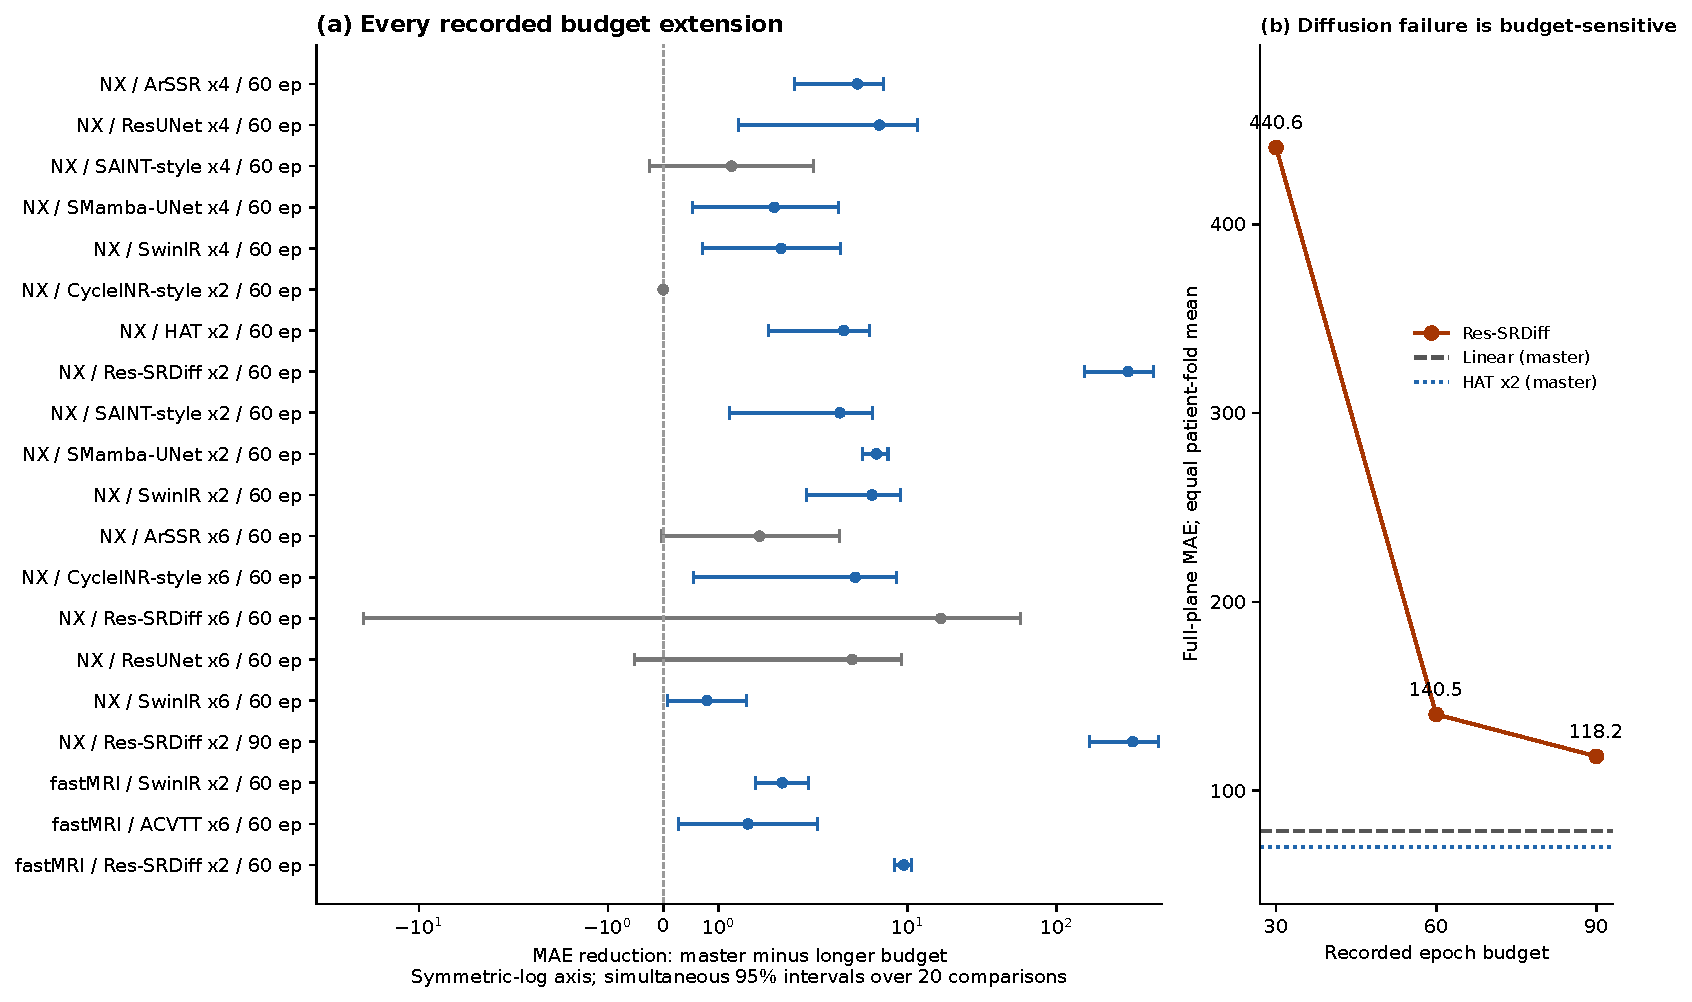
\includegraphics[width=\textwidth]{p15_training_budget.pdf}
\caption{All 20 recorded budget extensions. Positive reductions favor longer training; the symmetric-log axis keeps the large diffusion changes and small effects visible. Intervals simultaneously cover the 20 primary MAE contrasts. Five cross zero. Budget sensitivity does not validate a new QA score or erase the original short-budget failure.}
\end{figure*}


\subsection{Preserved common-support reconstruction benchmark}
\begin{table*}[t]
\caption{fastMRI recovered reconstruction context. Four metrics at every available factor; ``--- denotes unavailable audited cells.}
\label{tab:arch-benchmark}\centering\scriptsize
\setlength{\tabcolsep}{3pt}
\begin{tabular}{lrrrrrrrrrrrr}
\toprule
&\multicolumn{4}{c}{$\times2$}&\multicolumn{4}{c}{$\times4$}&\multicolumn{4}{c}{$\times6$}\\
Method&MAE&PSNR&SSIM&NCC&MAE&PSNR&SSIM&NCC&MAE&PSNR&SSIM&NCC\\
\midrule
Linear & 98.66 & 16.77 & 0.7707 & 0.7816 & 134.54 & 14.24 & 0.5884 & 0.5953 & 148.66 & 13.42 & 0.5042 & 0.5098 \\
Cubic & 114.51 & 15.63 & 0.7432 & 0.7414 & 153.24 & 13.21 & 0.5443 & 0.5411 & 148.66 & 13.42 & 0.5042 & 0.5098 \\
ACSI-Net & --- & --- & --- & --- & --- & --- & --- & --- & --- & --- & --- & --- \\
ACVTT & 97.73 & 16.94 & 0.7794 & 0.7911 & 122.23 & 15.38 & 0.6676 & 0.6886 & 124.63 & 15.00 & 0.6264 & 0.6485 \\
ArSSR & 80.03 & 18.19 & 0.8342 & 0.8506 & 114.21 & 15.38 & 0.6659 & 0.6888 & 128.03 & 14.51 & 0.5814 & 0.6057 \\
CycleINR & 80.25 & 18.17 & 0.8346 & 0.8496 & 114.39 & 15.38 & 0.6659 & 0.6888 & 128.25 & 14.47 & 0.5774 & 0.6033 \\
HAT & 68.03 & 19.59 & 0.8909 & 0.8940 & 86.09 & 17.80 & 0.8277 & 0.8327 & 96.75 & 16.82 & 0.7727 & 0.7826 \\
I3Net & 45.61 & 22.57 & 0.9459 & 0.9473 & 70.87 & 19.03 & 0.8714 & 0.8757 & 81.61 & 17.82 & 0.8256 & 0.8333 \\
Pix2PixGAN & 56.64 & 20.91 & 0.9204 & 0.9220 & 92.41 & 16.95 & 0.8076 & 0.8067 & 95.61 & 16.61 & 0.7913 & 0.7911 \\
Res-SRDiff & 89.32 & 17.49 & 0.8203 & 0.8272 & 95.98 & 16.75 & 0.7781 & 0.7865 & 102.11 & 16.22 & 0.7655 & 0.7655 \\
ResUNet & 72.73 & 19.12 & 0.8785 & 0.8814 & 92.68 & 17.27 & 0.8014 & 0.8087 & 92.93 & 17.14 & 0.7940 & 0.8013 \\
SAINT & 72.08 & 19.31 & 0.8857 & 0.8874 & 80.14 & 18.30 & 0.8477 & 0.8511 & 90.87 & 17.35 & 0.8071 & 0.8116 \\
SMamba-UNet & 67.94 & 19.52 & 0.8887 & 0.8916 & 85.88 & 17.68 & 0.8194 & 0.8267 & 97.94 & 16.86 & 0.7741 & 0.7849 \\
SwinIR & 65.69 & 19.78 & 0.8948 & 0.8978 & 90.37 & 17.37 & 0.8028 & 0.8121 & 97.73 & 16.83 & 0.7725 & 0.7835 \\
\bottomrule
\end{tabular}
\end{table*}
\begin{table*}[t]
\caption{IXI recovered reconstruction context. Four metrics at every available factor; ``--- denotes unavailable audited cells.}
\label{tab:arch-benchmark-ixi}\centering\scriptsize
\setlength{\tabcolsep}{3pt}
\begin{tabular}{lrrrrrrrrrrrr}
\toprule
&\multicolumn{4}{c}{$\times2$}&\multicolumn{4}{c}{$\times4$}&\multicolumn{4}{c}{$\times6$}\\
Method&MAE&PSNR&SSIM&NCC&MAE&PSNR&SSIM&NCC&MAE&PSNR&SSIM&NCC\\
\midrule
Linear & --- & --- & --- & --- & 65.99 & 20.34 & 0.9003 & 0.9030 & --- & --- & --- & --- \\
Cubic & --- & --- & --- & --- & 69.87 & 19.99 & 0.8984 & 0.8977 & --- & --- & --- & --- \\
ACSI-Net & --- & --- & --- & --- & 47.13 & 23.12 & 0.9480 & 0.9482 & --- & --- & --- & --- \\
ACVTT & --- & --- & --- & --- & --- & --- & --- & --- & --- & --- & --- & --- \\
ArSSR & --- & --- & --- & --- & --- & --- & --- & --- & --- & --- & --- & --- \\
CycleINR & --- & --- & --- & --- & --- & --- & --- & --- & --- & --- & --- & --- \\
HAT & --- & --- & --- & --- & 50.18 & 22.51 & 0.9414 & 0.9413 & --- & --- & --- & --- \\
I3Net & --- & --- & --- & --- & 39.26 & 25.03 & 0.9645 & 0.9644 & --- & --- & --- & --- \\
Pix2PixGAN & --- & --- & --- & --- & --- & --- & --- & --- & --- & --- & --- & --- \\
Res-SRDiff & --- & --- & --- & --- & --- & --- & --- & --- & --- & --- & --- & --- \\
ResUNet & --- & --- & --- & --- & --- & --- & --- & --- & --- & --- & --- & --- \\
SAINT & --- & --- & --- & --- & --- & --- & --- & --- & --- & --- & --- & --- \\
SMamba-UNet & --- & --- & --- & --- & --- & --- & --- & --- & --- & --- & --- & --- \\
SwinIR & --- & --- & --- & --- & 50.55 & 22.46 & 0.9406 & 0.9404 & --- & --- & --- & --- \\
\bottomrule
\end{tabular}
\end{table*}
\begin{table*}[t]
\caption{NingXia recovered reconstruction context. Four metrics at every available factor; ``--- denotes unavailable audited cells.}
\label{tab:arch-benchmark-ningxia}\centering\scriptsize
\setlength{\tabcolsep}{3pt}
\begin{tabular}{lrrrrrrrrrrrr}
\toprule
&\multicolumn{4}{c}{$\times2$}&\multicolumn{4}{c}{$\times4$}&\multicolumn{4}{c}{$\times6$}\\
Method&MAE&PSNR&SSIM&NCC&MAE&PSNR&SSIM&NCC&MAE&PSNR&SSIM&NCC\\
\midrule
Linear & 136.78 & 18.12 & 0.7611 & 0.7697 & 175.93 & 16.14 & 0.6350 & 0.6408 & 201.72 & 15.02 & 0.5343 & 0.5378 \\
Cubic & 153.41 & 17.29 & 0.7423 & 0.7412 & 197.41 & 15.20 & 0.5998 & 0.5968 & 204.51 & 14.92 & 0.5298 & 0.5329 \\
ACSI-Net & --- & --- & --- & --- & --- & --- & --- & --- & --- & --- & --- & --- \\
ACVTT & 131.78 & 18.45 & 0.7711 & 0.7850 & 162.77 & 16.85 & 0.6640 & 0.6832 & 185.36 & 15.89 & 0.5626 & 0.5881 \\
ArSSR & 133.56 & 18.28 & 0.7662 & 0.7773 & 165.77 & 16.51 & 0.6509 & 0.6655 & 186.41 & 15.57 & 0.5523 & 0.5704 \\
CycleINR & 133.56 & 18.28 & 0.7662 & 0.7773 & 172.33 & 16.30 & 0.6417 & 0.6501 & 198.16 & 15.15 & 0.5400 & 0.5466 \\
HAT & 122.16 & 18.91 & 0.7963 & 0.8082 & 149.41 & 17.25 & 0.6961 & 0.7153 & 172.24 & 16.23 & 0.5903 & 0.6229 \\
I3Net & 124.09 & 18.82 & 0.7860 & 0.8046 & 162.62 & 16.80 & 0.6332 & 0.6836 & 188.46 & 15.65 & 0.5102 & 0.5723 \\
Pix2PixGAN & 129.67 & 18.35 & 0.7744 & 0.7855 & 183.70 & 15.73 & 0.6094 & 0.6177 & 218.87 & 14.43 & 0.4596 & 0.4733 \\
Res-SRDiff & 479.32 & 10.40 & 0.5459 & 0.6322 & 225.44 & 14.93 & 0.5519 & 0.5661 & 254.89 & 13.91 & 0.4379 & 0.4685 \\
ResUNet & 132.33 & 18.40 & 0.7697 & 0.7828 & 164.52 & 16.77 & 0.6620 & 0.6785 & 180.15 & 16.01 & 0.5812 & 0.6030 \\
SAINT & 130.89 & 18.48 & 0.7742 & 0.7876 & 154.55 & 17.15 & 0.6904 & 0.7069 & 186.94 & 15.89 & 0.5670 & 0.5960 \\
SMamba-UNet & 129.36 & 18.57 & 0.7764 & 0.7906 & 150.46 & 17.22 & 0.6868 & 0.7091 & 176.48 & 16.17 & 0.5814 & 0.6161 \\
SwinIR & 127.41 & 18.67 & 0.7829 & 0.7961 & 148.66 & 17.27 & 0.6975 & 0.7152 & 172.19 & 16.20 & 0.5853 & 0.6202 \\
\bottomrule
\end{tabular}
\end{table*}

